\section[Introduction]{Introduction\footnote{All code that creates the evidence for this chapter can be found here: \url{https://github.com/apmoore1/tdsa_comparisons}. Certain sections throughout this chapter may have more specific pointers to python notebooks that created the analyses within that given section.}}
\label{section_case_intro}
Following on from chapter \ref{chapter:methodology}, several case studies will be explored using the newly developed TDSA evaluation methodology to test if it can quantify the justification behind these new developments. These justifications are normally qualitative case studies which are hard to quantify and to a large extent impossible to compare. Thus the importance on testing if this new TDSA evaluation methodology can work in practice is highly motivated to overcome the issues with qualitative analysis. Furthermore in each case study a rigorous experimental setup\footnote{This is through statistical testing, comparing across more models and datasets, and in the inter-target encoding setup comparing to a more suitable baseline model.} will be conducted unlike many previous works.

The new developments, where each is a separate case study within the chapter, within the TDSA literature that will be tested are; encoding the target's position (position encoding) \citep{gu-etal-2018-position}, inter-target encoding where each target is aware of all of targets within the same text \citep{hazarika-etal-2018-modeling}, and CWR \citep{sun-etal-2019-utilizing,xu-etal-2019-bert}. Of these developments, only the first two are TDSA specific whereas the transfer learning is a general machine learning concept that has been shown useful in many NLP tasks \citep{peters-etal-2018-deep}. These developments have been mainly justified by the improvements on the overall accuracy and/or macro F1 score, but the justification in the paper is normally more detailed. An example justification (and one that is typical of most developments) of inter-target encoding from \citet{hazarika-etal-2018-modeling}, where they first show improvements on the general accuracy scores over baselines. They then further state these improvements are due to the model being able to infer one target's sentiment from knowing another target's sentiment, and show this through a case study (section 4.2) from a few samples. The reason for inter-target encoding does sound valid but the case studies are qualitative and thus hard to quantify and compare too. Furthermore in both position and inter-target encoding there have been papers by \citet{he-etal-2018-exploiting} and \citet{majumder-etal-2018-iarm} that respectively use more detailed quantitative metrics through their own error splits to justify these improvements. However the error splits used in both cases (\textit{NT}) have been shown within chapter \ref{chapter:methodology} to be unsuitable.

All of these new developments will be applied to the methods that were used within chapter \ref{chapter:methodology}, as these methods can easily be enhanced with these new developments. Furthermore the same experimental setup that was used within chapter \ref{chapter:methodology}, described in section \ref{section:aug_experimental_setup}, will be used throughout this chapter.

%Furthermore within the TDSA literature there have been many general developments with regards to improvements that are to some extent agnostic to the Neural Network (NN) architecture they are applied to. The general developments of note for this chapter are; encoding the target's position (position encoding) \citep{gu-etal-2018-position}, inter-target encoding where each target is aware of all of targets within the same text \citep{hazarika-etal-2018-modeling}, and transfer learning from Bi-directional Language Models (BiLM) \citep{sun-etal-2019-utilizing,xu-etal-2019-bert} (also known as Contextualised Word Representations (CWR) which is what they will be called from now on). Of these developments, only the first two are TDSA specific where as the transfer learning is a general machine learning concept that has been shown useful in many NLP tasks \citep{peters-etal-2018-deep}. These developments have been mainly justified by the improvements on the overall accuracy and/or macro F1 score, but the justification in the paper is normally more detailed. An example justification (and one that is typical of most developments) of inter-target encoding from \citet{hazarika-etal-2018-modeling}, where they first show improvements on the general accuracy scores over baselines. They then further state these improvements are due to the model being able to infer one target's sentiment from knowing another target's sentiment, and show this through a case study (section 4.2) from a few samples. The reason for inter-target encoding does sound valid and the case studies do help this, however qualitative case studies are hard to quantify from these papers and to a large extent impossible to compare. Furthermore in both position and inter-target encoding there have been papers by \citet{he-etal-2018-exploiting} and \citet{majumder-etal-2018-iarm} that respectively use more detailed quantitative metrics through their own error splits to justify these improvement. However the error splits used in both cases are shown within this chapter to be unsuitable as they both measure other factors that the original authors did not know they were measuring.
%Furthermore as stated in the introduction section \ref{section:aug_introduction}, the TDSA methods will be enhanced with three different developments; 1. position-encoding, 2. inter-target encoding, and 3. CWR. From the three methods, only \textit{IAN} and \textit{Att-AE} will be enhanced with position-encoding as \textit{TDLSTM} already has the target position somewhat encoded into its NN architecture. Each of these enhancements will be tested against their standard/base model with respect to the error analysis splits. The quantitative results from these error analysis splits will be compared to the original qualitative justifications for these developments from the respective papers.
% Finally these three baseline TDSA models are then enhanced (when appropriate) with position encoding, inter-target encoding, and CWR to quantify how these different developments enhance the models through the error splits. The results from these splits and metrics for the position and inter-target encoding enhancements will for the first time quantify the theory behind the developments, and in contrast to previous work, we use suitable error analysis splits and a more rigorous experimental setup\footnote{This is through statistical testing, comparing across more models and datasets, and in the inter-target encoding setup comparing to a more suitable baseline model.}. The results from the CWR will be the first detailed quantifiable results that should highlight what the models are not capturing and should help guide future state-of-the-art TDSA models. 
\section[Position Encoding]{Position Encoding\footnote{All graphs within this section have been generated through the following notebook \url{https://github.com/apmoore1/tdsa_comparisons/blob/master/analysis/Position_Encoding.ipynb}.}}
\label{section:aug_position_encoding}
\subsection{Introduction}
This is the first model enhancement that will be explored in this chapter. As stated in the introduction section \ref{section:aug_method_performance_intro}, the two models that will be explored in this section are \textit{IAN} and \textit{Att-AE} due to the \textit{TDLSTM} already having position information somewhat encoded into its NN architecture. Within the prior work, position information has been encoded into different TDSA methods in broadly three different approaches; weighting, embedding, and via the construction of the NN architecture (construction). Position weighting is probably the simplest approach as it weights the vectors of tokens/words\footnote{Normally after they have been encoded via some sequence encoder e.g. LSTM.} based on some distance metric to the relevant target word(s). However there is no one standard distance metric in the literature but a lot of them are very similar; \citet{chen-etal-2017-recurrent} (equation 7 and section 3.3) based the weighting on how many tokens are between the context word and the nearest target word (token) and then normalised via sentence length\footnote{They further encoded the relative position of the word into the model.}. Other methods have created an arbitrary cut off so that context words that are too distant are ignored \citep{he-etal-2018-exploiting, zhao2019modeling}, \citet{zhang-etal-2019-aspect} uses the same weighting as \citet{chen-etal-2017-recurrent} but ignores the target words. \citet{he-etal-2018-exploiting} incorporated syntax into the weighting where the position to the target word(s) is defined by the distance through the dependency tree. Lastly \citet{li-etal-2018-transformation} used the same weighting as \citet{chen-etal-2017-recurrent} but normalises using an arbitrary constant rather than the sentence length ($n$).  In most cases across all of the experiments within the prior work on position weighting when the work has shown ablation studies position weighting has increased the performance of the models\footnote{The only work that has shown position weighting to harm performance is \citet{zhang-etal-2019-aspect} on the Twitter and Rest14 datasets in table 3.}. Position embeddings unlike the weighting mechanism encodes the position of a token/word via a learnt embedding space. Position embeddings are similar to the weighting mechanism in that they create position indexes that are relative to the target, where the indexes are created similar to the weighting mechanism. These position indexes for each word are calculated based on token distance from the closest target word. These position indexes, unlike the weighting method, are integers not floats as these integers are then used as an index to the random initialised (position) embedding. These position embeddings are then normally concatenated onto the word embeddings that represent the tokens in the sentence that the target occurs in \citep{gu-etal-2018-position, li-etal-2018-hierarchical, chen-qian-2019-transfer, sun-etal-2019-aspect, kumar2020aspect}. Unlike the position weighting literature all prior works that have used position embeddings calculate the position indexes based on relative distance to the nearest target token. Out of the five prior works, three use a position embedding dimension of 100, one uses 50, and another 30\footnote{Another prior work does not state the dimension of the position embeddings \citep{du-etal-2019-capsule}.}.  For clarification on position weighting and embeddings, table \ref{tab:aug_examples_position_indexes_weighting} shows an example text that has been tokenised where the target that is being predicted for is `Apple Mac', beneath each token is the weighting value and position index where the weighting value is calculated using equation \ref{eq:aug_chen_position}, which has come from \citet{chen-etal-2017-recurrent}. In equation \ref{eq:aug_chen_position}, $i$ represents the index of the token/word whose position is to be weighted, $\tau$ represents the index of the closest target token to $i$, and $n$ is the length of the text in tokens. 

\begin{equation}
    w_i = 1 - \frac{|\tau - i|}{n}
    \label{eq:aug_chen_position}
\end{equation}

\begin{table}[!h]
    \centering
    \begin{tabular}{|c|c|c|c|c|c|}
    \hline
         Tokens: & The & Apple & Mac & is & great  \\
    \hline
         Position indexes & 1 & 0 & 0 & 1 & 2 \\
    \hline
         Position weighting & 0.8 & 1 & 1 & 0.8 & 0.6 \\
    \hline
    \end{tabular}
    \caption{Example text which contains the target `Apple Mac', where the text has been tokenised and the associated position indexes and weightings are shown.}
    \label{tab:aug_examples_position_indexes_weighting}
\end{table}

Construction based approaches have used numerous different NN methods. \citet{tang-etal-2016-effective} (\textit{TDLSTM}) used RNNs where a forward RNN would process all tokens up to the last target token and a backward RNN for all tokens to the first target token. Other approaches have split the sentence up into left, right, and target contexts and aggregated the word embeddings using Neural Pooling methods \citep{vo2015target, zhang2016gated} or using a RNN based sequence encoder \citep{liu-zhang-2017-attention}. Another direction is to make use of a dependency parser to explicitly model the syntactic structure of the target's position, \citet{dong-etal-2014-adaptive} re-ordered the dependency tree to ensure the target word is the root and then used a Recursive NN (RCNN). \citet{sun-etal-2019-aspect, huang-carley-2019-syntax} both use the dependency tree without re-ordering it and apply a Graph NN (GNN) to encode words that are close to the target word through the dependency tree. \citet{nguyen-shirai-2015-phrasernn} used both a dependency and constituency parser to create a phrase dependency tree where the the tree is re-ordered such that the target word phrase is always at the root of the tree, they then used a RCNN to encode the tree data. Lastly one prior work has combined both position embeddings and a position based architecture \citep{sun-etal-2019-aspect}.

From this prior literature, the main reason for using position information is to create a more explicit bias in the model. The bias assumes that words that are closer to the target word(s) are more important and therefore should be given more weight, attention, or priority in the model. This bias is more or less explicit depending on the method used, in the case of weighting it is more explicit as words that are closer are always weighted higher than those further away. In comparison the embedding approach can be less biased as it allows the model to chose what words are closer and more important through the embedding. The construction method is hard to compare to the embedding and weighting approaches on bias as these approaches to some degree change their whole model so that position information is prioritised. In the case of \textit{TDLSTM} \citep{tang-etal-2016-effective} the bias of relatively close words are prioritised, compared to \citet{dong-etal-2014-adaptive} where they prioritise the syntactic distance between tokens and the targets words. 

In general, encoding position information is used to improve the performance on sentences that contain multiple targets as it should help match relevant words with their respective target \citep{li-etal-2018-hierarchical, he-etal-2018-exploiting}. This indicates that the point of position encoding is help improve target sentiment relation modelling. From these position encoding papers \citet{he-etal-2018-exploiting} is the only one to quantitatively evaluate the importance of position information further than just using overall metrics on the entire dataset. \citet{he-etal-2018-exploiting} have shown that using syntactic position weighting improves the performance for sentences that contain more than one target. The way this was evaluated was in effect using the \textit{NT} splits where they subsetted the data based on 1, 2, 3, and more than 3 targets per text. As has been shown in the last subsection \ref{section:aug_baseline} that the performance on the \textit{NT} split tends to be dominated by sentiment factors and does not directly measure target sentiment relationships. Even though \citet{he-etal-2018-exploiting} has performed a good quantitative evaluation, this cannot determine if the position information is actually improving target sentiment relation modelling. Therefore in this section position encoding will be evaluated across the two TDSA methods using the recommended error splits from the last subsection \textit{DS} and \textit{TSR} as well as using the TDSA specific metrics \textit{STAC Multi} and \textit{STAC 1}. In doing so, position encoding will be thoroughly evaluated for target sentiment relation modelling that it is claimed to do from the literature, as well as exploring any other positive or negative side affects. Furthermore the \textit{NT} subsets will also be included in the evaluation to demonstrate the point of why this split is not suitable for error analysis as it has been used in the prior work \citep{he-etal-2018-exploiting}. 

Given this prior literature the position encoding that will be used in this section is position weighting. This was chosen as it requires no extra parameters unlike the position embeddings and does not require fundamentally changing the NN architecture. The distance metric proposed by \citet{chen-etal-2017-recurrent} as shown in equation \ref{eq:aug_chen_position} will be used as it does not require any arbitrary cut off or normalising parameter to be tuned \citep{zhao2019modeling, li-etal-2018-transformation}, nor does it mask any words \citep{zhang-etal-2019-aspect}, and finally does not require a dependency parser \citep{he-etal-2018-exploiting}. Furthermore as this weighting method does not remove any words it allows the model to ignore the explicit bias of the position weighting in cases where the closest words are not always the most important e.g. in the case that the affecting opinion word(s) are a few syntactic hops away from the target. The position weighting will be applied to the context/sentence vectors after being encoded by the LSTM layer and before the attention is applied in both \textit{IAN} and \textit{Att-AE}.

\subsection{Experiments}

Figure \ref{fig:aug_overall_position_scores} shows the overall scores of the position encoded \textit{IAN} and \textit{Att-AE} models. These scores are somewhat meaningless without comparing them to their respective non-position encoded baseline models.

\begin{figure}[h!]
    \centering
    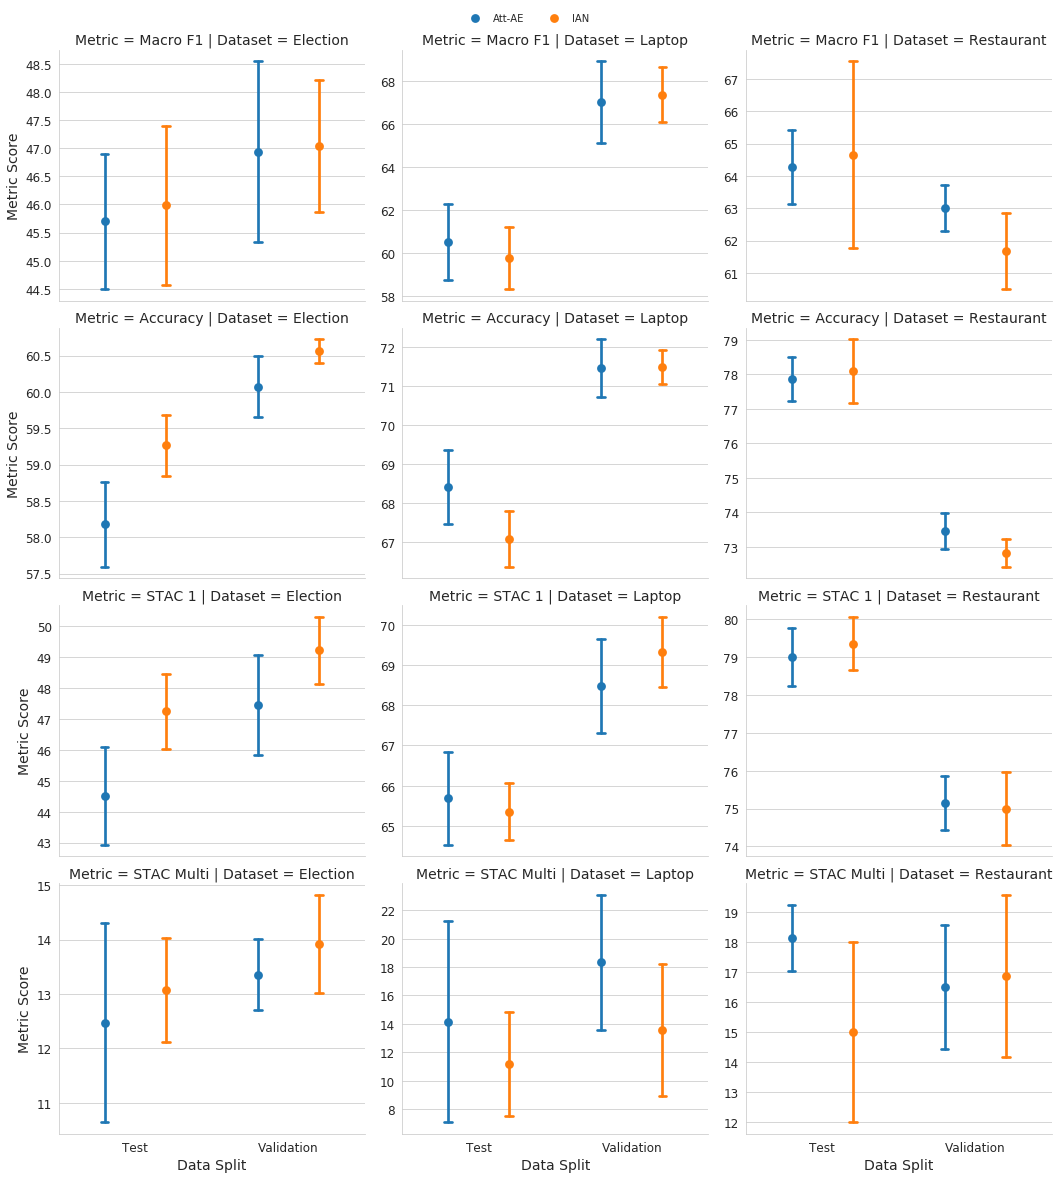
\includegraphics[scale=0.32]{images/augmentation/methods_performance/Position_Encoding/overall_position_scores.png}
    \caption{Columns represent different datasets, rows different metrics. Each plot represents the two position encoded models metric score on the test and validation splits.}
    \label{fig:aug_overall_position_scores}
\end{figure}

Figure \ref{fig:aug_position_baseline_overall_differences} shows the metric score difference between the position and the respective baseline models. As we can see from the results the overall trend is that, no matter the dataset or metric, position weighting on average improves the models performance. There are a few exceptions to this the \textit{STAC 1} results for both Election and Laptop datasets, and the \textit{accuracy} metric for the Laptop dataset. Furthermore there are several results where even though the mean is positive the standard deviations are so large that they go into the negative of the metric score difference. This shows that the trend might show an overall improvement in performance but the improvement is marginal.

%Finally the metric that appears to have the largest benefit from position weighting is the \textit{STAC-Multi} which does suggest that position weighting does improve the target sentiment relationship modelling, confirming the hypothesis from the literature about position weighting. Further this may explain the reason why \textit{TDLSTM} performed consistently better than the rest in the baseline results for the \textit{STAC-Multi} metric (see figure \ref{fig:baseline_stac_scores.png}) due to it having position information encoded into it NN architecture.

\begin{figure}[h!]
    \centering
    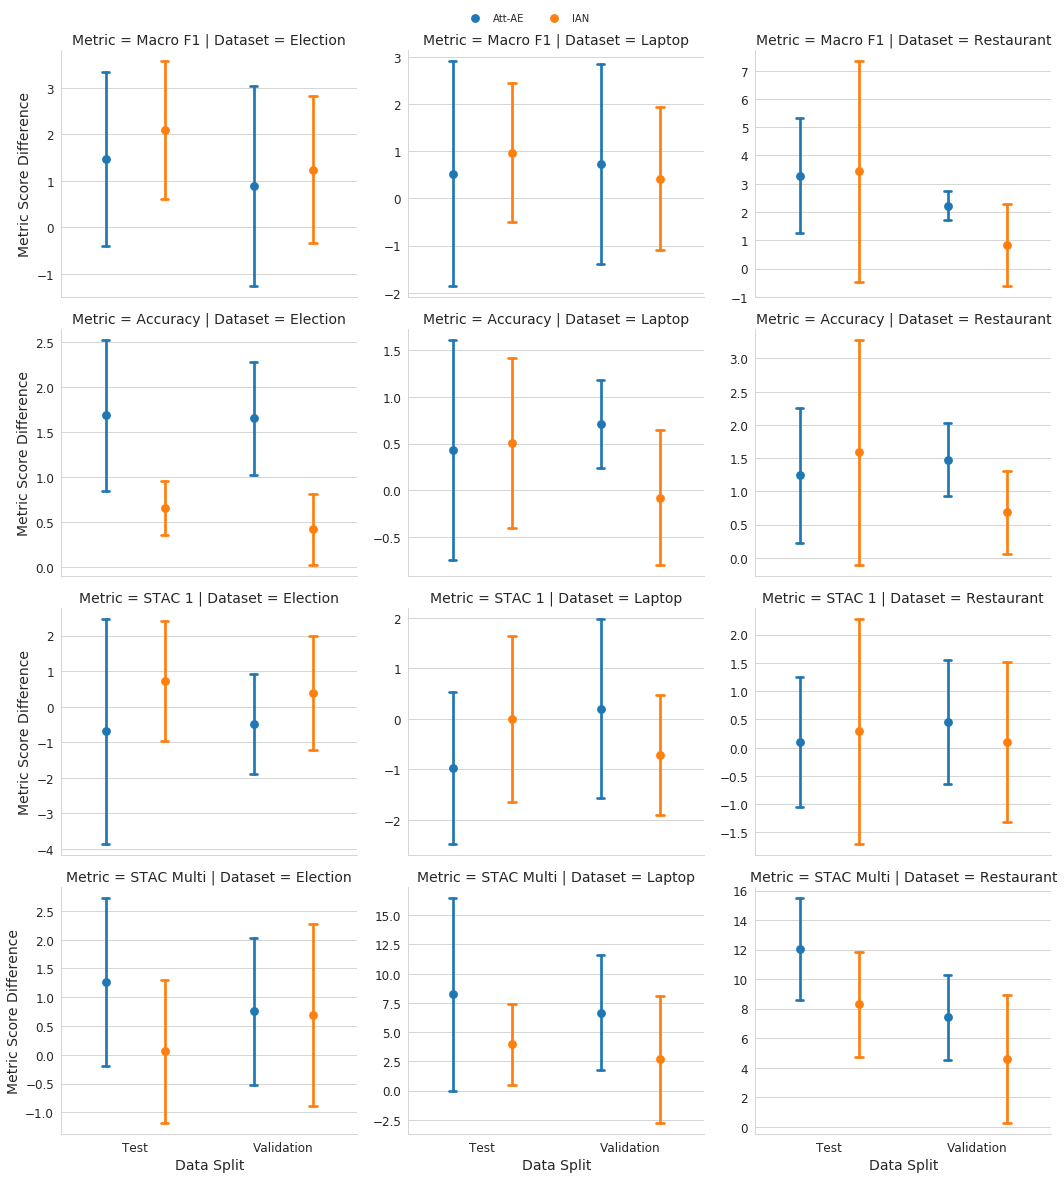
\includegraphics[scale=0.32]{images/augmentation/methods_performance/Position_Encoding/position_baseline_overall_differences.png}
    \caption{Columns represent different datasets, rows different metrics. Each plot represents the differences between the position and baseline models for the relevant metric score on the test and validation splits.}
    \label{fig:aug_position_baseline_overall_differences}
\end{figure}

To better visualise the differences figures \ref{fig:aug_position_overall_sig_models} and \ref{fig:aug_position_corrected_overall_sig_models} show the number of models that are significantly better than their baseline, where the former is not corrected for multiple significance tests where as the later is using Bonferroni and is aggregated across datasets. There were no models on any of the metrics or dataset splits where the baseline models were significantly better than the position models. From these heatmaps it can indeed be seen that the Restaurant dataset does benefit the most.%\footnote{The p-values for comparing the position to their baseline models can be found in table and the baseline to the position models in table} 

As be seen from the heatmaps, the Laptop and the Restaurant datasets are the only datasets that consistently have position models that are significantly better on the \textit{STAC Multi} metric. Furthermore the Laptop dataset is the only dataset that does not find the position models to be consistently significantly better than the baselines on \textit{Accuracy}. This might not be a surprising finding considering that the Laptop dataset contains the least number of $DS_2$ and $DS_3$ samples relative to its size (see figure \ref{fig:aug_error_analysis_ds}). Thus as the findings suggest here that the position information improves the scores on the samples that have multiple unique sentiments within the sentences ($DS_2$ and $DS_3$), compared to a dataset that is made up of mainly sentences that only contain one unique sentiment. This reason is also related to another, of why position information does not perform significantly better on the \textit{STAC 1} metric. As the \textit{STAC 1} metric is only looking at the accuracy score for sentences that contain one unique sentiment and that the model predicts all samples in those sentences correctly. A model that overfits to the most frequent sentiment class will perform well on this metric. As the position information is biasing the model towards only looking at local context around the target it removes the bias for the model to look at the global context. This shows that biasing the model towards the local context through the position information removes some of the position overfitting that the baselines models exploited. It is clear to some degree that for at least the Laptop and Restaurant datasets that as the position models have improved on the \textit{STAC Multi} metric and not regressed on the \textit{STAC 1} metric, that the models are less prone to sentiment overfitting and do perform better at target sentiment relation modelling.

\begin{figure}[h!]
    \centering
    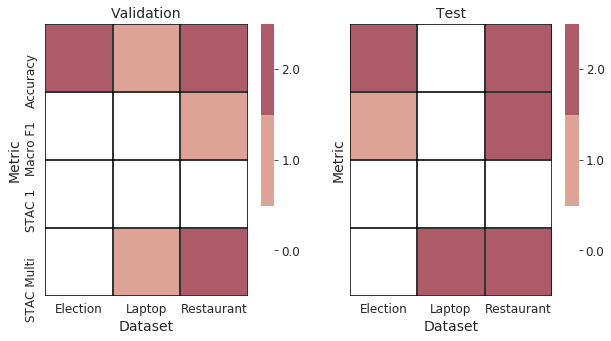
\includegraphics[scale=0.5]{images/augmentation/methods_performance/Position_Encoding/position_overall_sig_models.png}
    \caption{Heatmaps that represent the number of position models that are statistically significantly better than their baseline equivalents at the 95\% confidence level.}
    \label{fig:aug_position_overall_sig_models}
\end{figure}

\begin{figure}[h!]
    \centering
    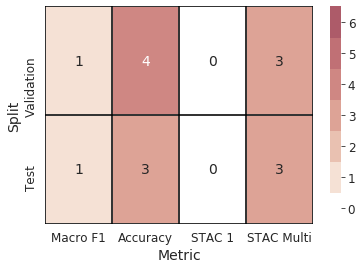
\includegraphics[scale=0.6]{images/augmentation/methods_performance/Position_Encoding/position_corrected_overall_sig_models.png}
    \caption{Heatmaps that represent the number of position models that are statistically significantly better than their baseline equivalents across all datasets at the 95\% confidence level. Where the multiple hypothesis tests have been corrected using Bonferroni.}
    \label{fig:aug_position_corrected_overall_sig_models}
\end{figure}

Furthermore from the heatmap results we can see that the Election dataset is the only one that the models do not perform significantly better than the baseline version on the \textit{STAC Multi} metric. However they do consistently perform better on the \textit{Accuracy} metric. This may suggest that the position information does improve the target sentiment relationship modelling but cannot be shown through the \textit{STAC Multi} metric as it requires all targets in the sentence to be correctly classified. The further reason why it is believed that it is improving the target sentiment relationship modelling rather than overfitting to the overall sentiment as the \textit{STAC 1} metric has not improved on the dataset. To investigate if the position models are improving the target sentiment relationship modelling on the Election dataset the results across all datasets for the \textit{DS}, \textit{TSR}, and \textit{NT} error splits are shown in figure \ref{fig:aug_position_split_difference_test_results} (\ref{fig:aug_position_split_difference_validation_results}) for the test (validation) split. The figure shows the difference between the position and respective baseline model\footnote{Figure \ref{fig:aug_position_split_overall_test_results} (\ref{fig:aug_position_split_overall_validation_results}) shows test (validation) results for the splits without subtracting from their respective baseline models.}. From this figure it is clear that that the position models improve the results for the $DS_2$ subset on the Restaurant and Laptop datasets. However for the Election dataset it would appear that the \textit{Att-AE} model is the one that benefits most from the position encoding (better seen in the validation results). The heatmaps in figure \ref{fig:aug_position_dataset_subset_heatmap} and \ref{fig:aug_position_combined_subset_heatmap}\footnote{The legend goes to $6$ as the number of position models that can be better than their baseline is $6$, as there are $2$ models and $3$ datasets per evaluation, and each model is evaluated against it's baseline across all datasets.} show the number of models that are significantly better than their baseline on each error subset, where the former is not corrected for multiple significance tests where as the later is using Bonferroni and is aggregated across datasets. The heatmaps differ by a large margin between the validation and test splits. The Laptop dataset from the validation split appears to be the only one that has no significant difference in any of the subsets, of which this differs from the overall metric results in figure showing that there is a significant difference for the \textit{STAC Multi} and \textit{Accuracy}. It can be seen for the Election dataset for both validation and test splits that for all subsets in the \textit{DS} split that a position model is significantly better. Furthermore when correcting for multiple hypothesis tests on the test split figure \ref{fig:aug_position_combined_subset_heatmap} shows that the Election dataset must contain at least one position model that is significantly better for the $DS_2$ and $DS_3$ subsets. This to some degree confirms that the position encoding must be improving the target sentiment relationship modelling even though it does not show through the \textit{STAC Multi} metric. This shows the reason why the \textit{DS} split is still useful as it shows a more fine grained analysis of the target sentiment relationship modelling. 

\begin{figure}[h!]
    \centering
    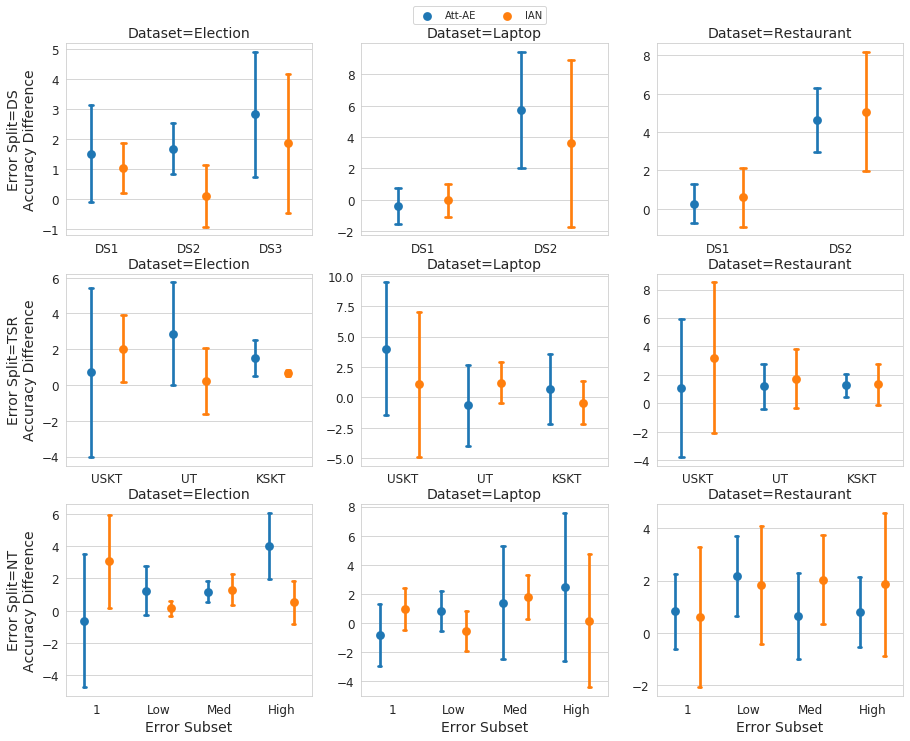
\includegraphics[scale=0.32]{images/augmentation/methods_performance/Position_Encoding/position_split_difference_test_results.png}
    \caption{Test split results. Columns represent different datasets, rows different error splits. Each plot represents the differences between the position and baseline models for the Accuracy metric on the given error subset.}
    \label{fig:aug_position_split_difference_test_results}
\end{figure}

\begin{figure}[h!]
    \centering
    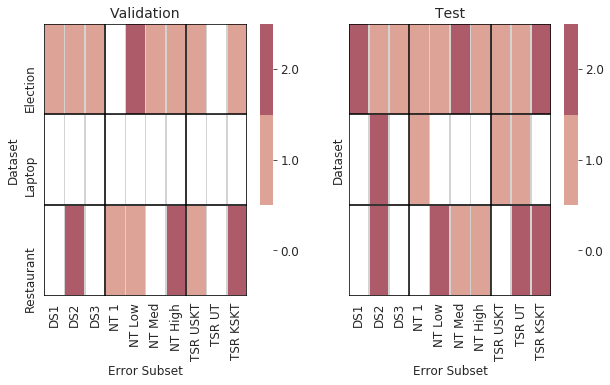
\includegraphics[scale=0.5]{images/augmentation/methods_performance/Position_Encoding/position_dataset_subset_heatmap.png}
    \caption{Heatmaps that represent the number of position models that are statistically significantly better than their baseline equivalents at the 95\% confidence level.}
    \label{fig:aug_position_dataset_subset_heatmap}
\end{figure}

\begin{figure}[h!]
    \centering
    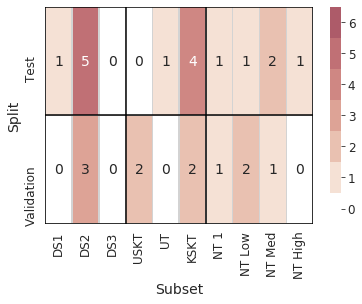
\includegraphics[scale=0.6]{images/augmentation/methods_performance/Position_Encoding/position_combined_subset_heatmap.png}
    \caption{Heatmaps that represent the number of position models that are statistically significantly better than their baseline equivalents across all datasets at the 95\% confidence level. Where the multiple hypothesis tests have been corrected using Bonferroni.}
    \label{fig:aug_position_combined_subset_heatmap}
\end{figure}

As was suggested in the last section \ref{section:aug_baseline} that the \textit{DS} and \textit{TSR} splits should be used when analysing the results, this is the reason why the \textit{TSR} split was included in the figures. From figure \ref{fig:aug_position_combined_subset_heatmap} for the \textit{TSR} split it can be seen that in general the only subset that the position models consistently perform better on is the \textit{KSKT} subset. This is most likely due to the target sentiment relationship modelling improvement, as the \textit{KSKT} subset is the dominate subset within the \textit{TSR} split (see figure \ref{fig:aug_error_analysis_trs}).

\begin{figure}[h!]
    \centering
    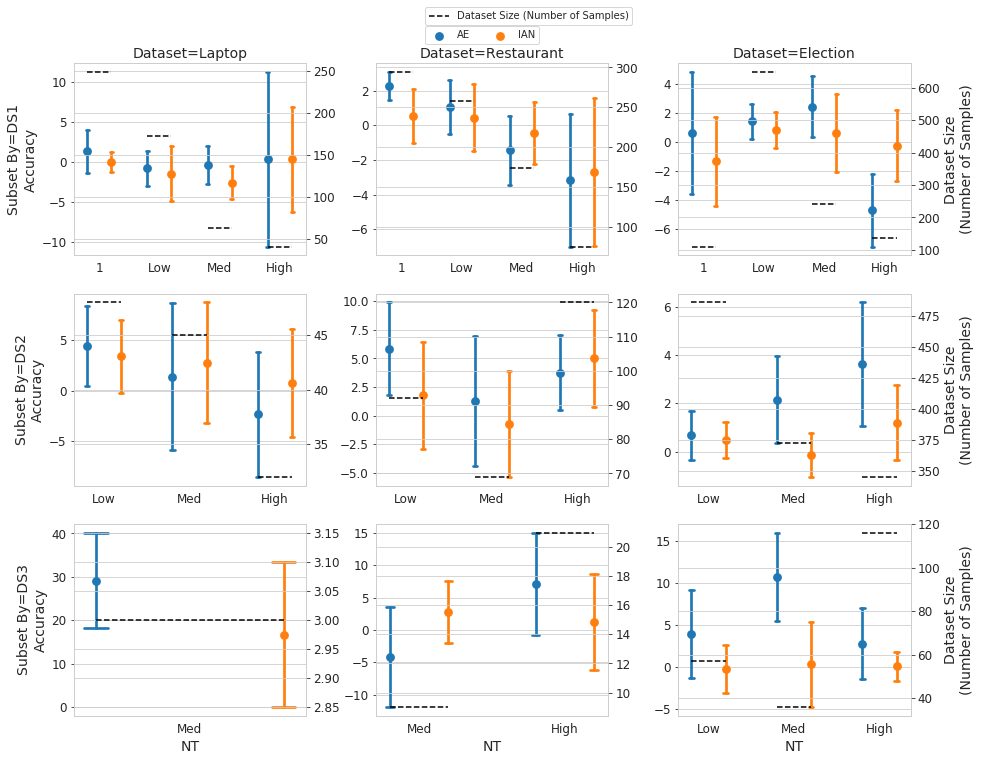
\includegraphics[scale=0.32]{images/augmentation/methods_performance/Position_Encoding/position_DS_NT_validation.png}
    \caption{Validation split results. Columns represent different datasets, rows different \textit{DS} error split subsets. Each plot represents the differences between the position and baseline models for the Accuracy metric on the given error subset.}
    \label{fig:aug_position_DS_NT_validation}
\end{figure}

\begin{figure}[h!]
    \centering
    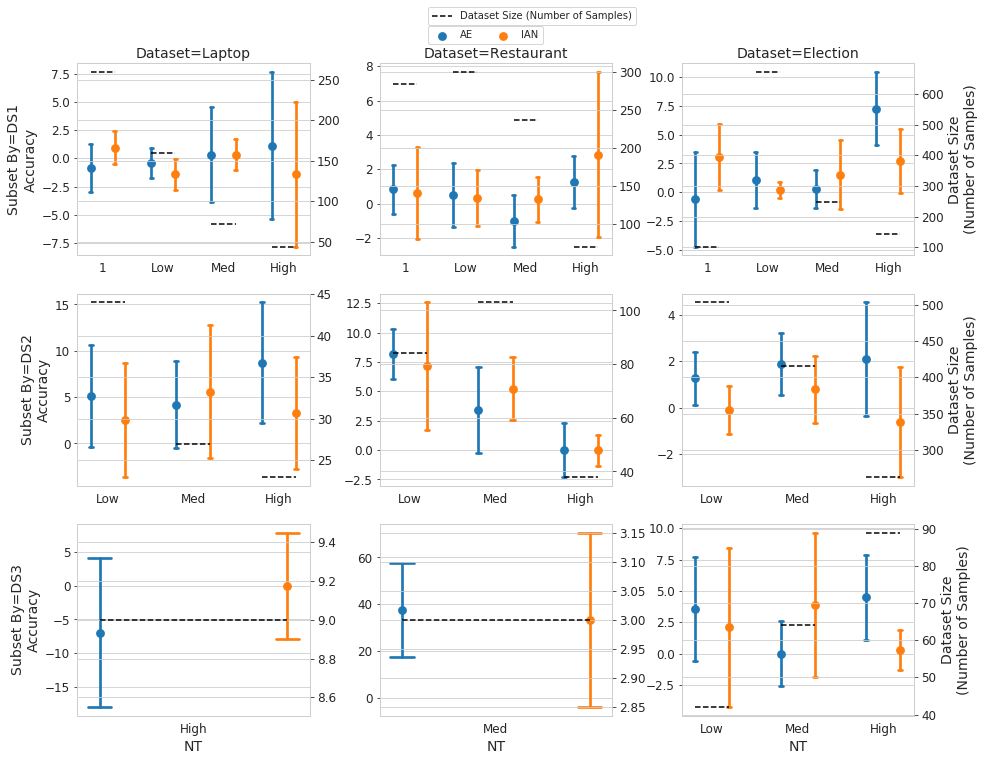
\includegraphics[scale=0.32]{images/augmentation/methods_performance/Position_Encoding/position_DS_NT_test.png}
    \caption{Test split results. Columns represent different datasets, rows different \textit{DS} error split subsets. Each plot represents the differences between the position and baseline models for the Accuracy metric on the given error subset.}
    \label{fig:aug_position_DS_NT_test}
\end{figure}

Lastly, as in the previous work by \citet{he-etal-2018-exploiting}, the way they evaluated the position encoding was through using a similar method to the \textit{NT} error splits. Therefore to show quantitatively that the \textit{NT} splits are not the best way to show that a method improves on target sentiment relationship modelling figure \ref{fig:aug_position_combined_subset_heatmap} finds that only a few models are significantly better across the different \textit{NT} subsets. When any of the \textit{NT} subsets are compared to the $DS_2$ subset none have more significant models. Furthermore, figures \ref{fig:aug_position_DS_NT_validation} and \ref{fig:aug_position_DS_NT_test} show the validation and test split performance difference between the position and baseline models when the data has been first subsetted by the \textit{DS} subsets (rows in the figures) and then further subsetted by the \textit{NT} subsets. From these figures it shows some in-consistencies of which the most of these are in the validation results. The validation results for the Restaurant dataset when subsetted by $DS_1$ show a large negative correlation of which this is most likely due to the baseline model being better a sentiment overfitting on sentences that contain lots of targets. Furthermore on the Laptop test and validation splits for the $DS_1$ subsetted row several of the results mean value is less than $0$ suggesting the baseline model is better in these circumstances. From across the test and validation splits out of all the $DS_1$ subsetted models $29.16\%$($\frac{14}{48}$) perform on average worse than their baseline models compared to $10.4\%$($\frac{5}{48}$) from the $DS_2$ and $DS_3$\footnote{The $DS_3$ subsetted models from the Laptop and Restaurant datasets where not included as they contain very few samples (less than $20$).} subsetted models. This to some degree shows that the \textit{NT} split for the $DS_1$ subsetted data at least is more likely measuring sentiment overfitting than target sentiment relationship modelling, as the baseline model perform competitively. From this it can be seen that when the number of targets does increase the performance of the position models do not always improve the results. Furthermore the \textit{NT} split is more affected by the sentiment factors within the sentence and can be skewed by sentiment overfitting.

\subsection{Conclusion}
This section has found that position encoding does improve TDSA models performance in general. Further it has been shown quantitatively that the theory from the literature on position encoding improving target sentiment relationship modelling \citep{li-etal-2018-hierarchical, he-etal-2018-exploiting} is true through the novel TDSA metrics (\textit{STAC Multi} and \textit{STAC 1}) and existing error split (\textit{DS}). This finding could explain the reason why the \textit{TDLSTM} model performed generally better than the others on the \textit{STAC Multi} metric, and $DS_2$ and $DS_3$ subsets within the baseline results section \ref{section:aug_baseline}. Lastly it has been shown again that the \textit{NT} split is not a useful error split to use due to it being skewed by sentiment overfitting. From this the results that \citet{he-etal-2018-exploiting} presented using a similar error analysis split as \textit{NT} does not quantitatively prove that position encoding does improve target sentiment relationship modelling. Therefore the results presented here are the first quantitative results demonstrating that position encoding does improve target sentiment relationship modelling.

\section[Inter-Target Encoding]{Inter-Target Encoding\footnote{All graphs within this section have been generated through the following notebook \url{https://github.com/apmoore1/tdsa_comparisons/blob/master/analysis/Aspect_Encoding.ipynb}.}}
\label{section:aug_inter_target_encoding}
\subsection{Introduction}
The majority of TDSA methods do not explicitly take into account other targets that may occur within the same sentence as the target that it is currently classifying, methods that do take this into account are target-aware. The standard non-target aware methods generally treat the problem as shown in figure \ref{fig:aug_normal_target_modelling}, where for each target (from the three) within the sentence is inputted into the (TDSA) model individually to create a target sentiment aware representation for the target (red/pink square), this representation is then projected down to a vector $\mathbb{R}^{c}$, where $c$ is the number of sentiment classes for prediction. Where as a target-aware model as shown in figure \ref{fig:aug_target_general_modelling} takes all of the targets as input and makes predictions on all targets (three of them in this case) in-affect at the same time, where the model explicitly makes itself aware of all targets within the text through the inter target encoding layer. The inter target encoding layer was first suggested by \citet{hazarika-etal-2018-modeling}, where they used an LSTM as their inter target encoder as shown in figure \ref{fig:aug_target_hazarika_modelling}. As can be seen the LSTM layer is uni-directional thus all targets preceding other targets within the sentence would not be aware of these future targets. This limitation was overcome in \citet{majumder-etal-2018-iarm} where they used a similar network to \citet{hazarika-etal-2018-modeling} but added a memory network on top, of which this memory network performed attention so that each target sentiment representation was aware of all other targets. \citet{zhao2019modeling} instead of using attention and an RNN structure made the targets aware of each other explicitly through a GNN as shown in figure \ref{fig:aug_target_zhao_modelling}. These inter target encoding layer methods is one of two general ways of making a model target aware. The other approach is through regularisation of the attention layer \citep{fan-etal-2018-multi} that is applied to the encoded word representations within the sentence, to make the representations target aware. This form of regularisation was called `Aspect Alignment Loss'\footnote{Aspect here is the same as target.} \citep{fan-etal-2018-multi}, where the intuition behind it was to penalise similar attention weight of targets in the same sentence that contain different sentiment\footnote{Equation 24 shows the Aspect Alignment Loss in \citet{fan-etal-2018-multi}.}. This was to try and force the attention weights of targets that have different sentiment to focus on different words within the sentence. The only other work that has used regularisation to make a model target aware is \citet{hu-etal-2019-constrained}. \citet{hu-etal-2019-constrained} applied a very similar technique to \citet{fan-etal-2018-multi}, however this work was done on the task of aspect based sentiment analysis rather than target\footnote{Aspect based in this thesis is the latent version of target based.}.

\begin{figure*}
        \centering
        \begin{subfigure}[b]{0.475\textwidth}
            \centering
            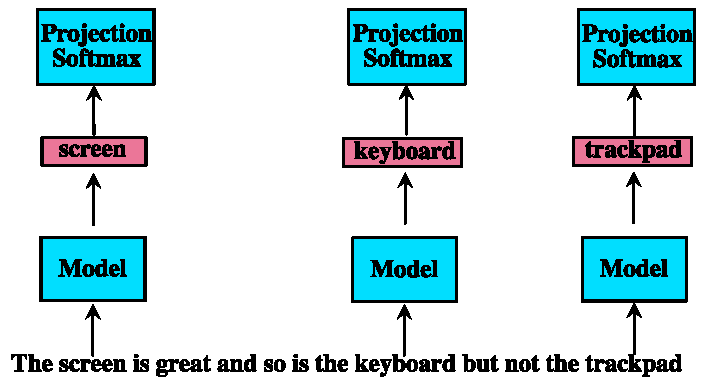
\includegraphics[width=\textwidth]{images/augmentation/methods_performance/Inter_Target/normal.pdf}
            \caption{General non-target aware setup.}    
            \label{fig:aug_normal_target_modelling}
        \end{subfigure}
        \hfill
        \begin{subfigure}[b]{0.475\textwidth}  
            \centering 
            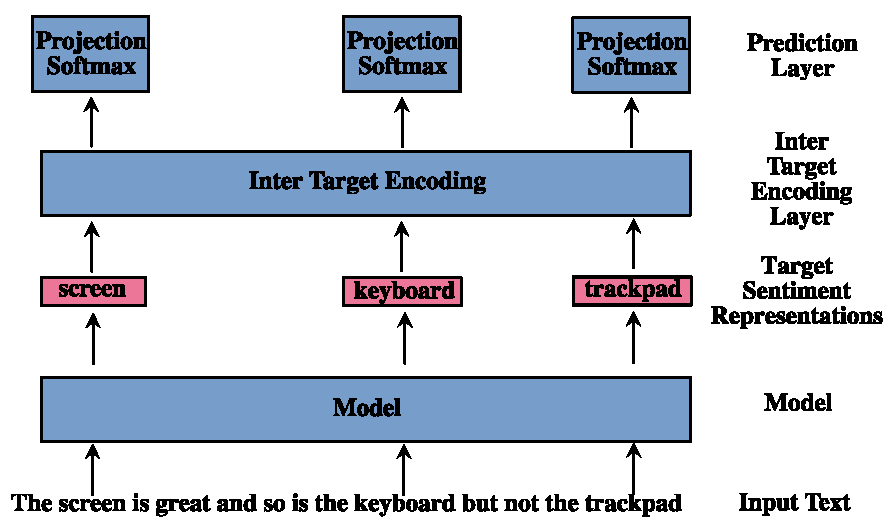
\includegraphics[width=\textwidth]{images/augmentation/methods_performance/Inter_Target/inter_target_encoding.pdf}
            \caption{General target aware setup.}    
            \label{fig:aug_target_general_modelling}
        \end{subfigure}
        \vskip\baselineskip
        \begin{subfigure}[b]{0.475\textwidth}   
            \centering 
            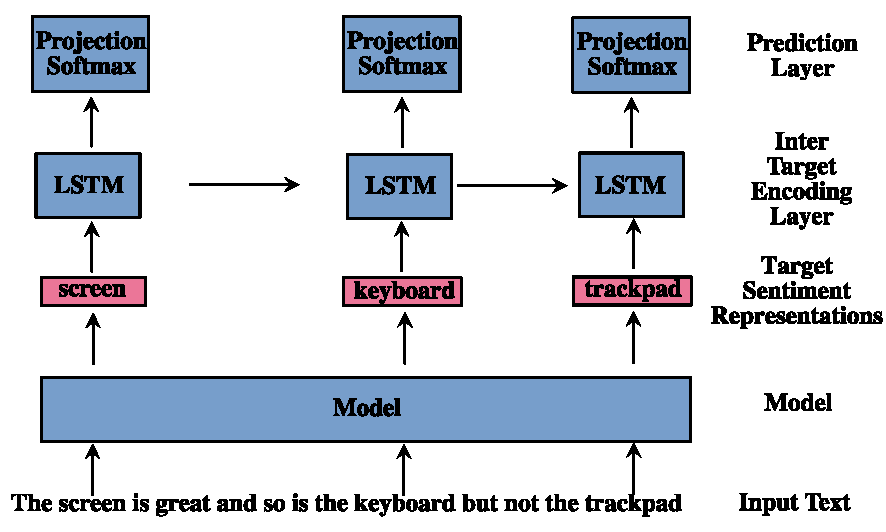
\includegraphics[width=\textwidth]{images/augmentation/methods_performance/Inter_Target/LSTM_Encdoing.pdf}
            \caption{Target aware setup of \citet{hazarika-etal-2018-modeling}.}    
            \label{fig:aug_target_hazarika_modelling}
        \end{subfigure}
        \quad
        \begin{subfigure}[b]{0.475\textwidth}   
            \centering 
            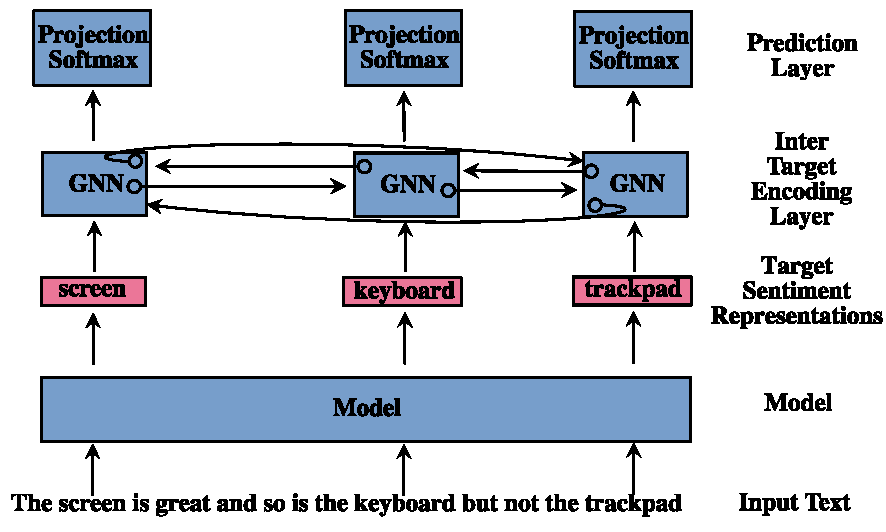
\includegraphics[width=\textwidth]{images/augmentation/methods_performance/Inter_Target/GNN_Encoding.pdf}
            \caption{Target aware setup of \citet{zhao2019modeling}.}    
            \label{fig:aug_target_zhao_modelling}
        \end{subfigure}
        \caption{The first row shows in abstract the difference between non target aware and aware setups. The second row shows more concrete target aware methods.} 
        \label{fig:aug_target_aware_and_non_setups}
\end{figure*}

The main benefit that these papers believe that the inter target encoding layer brings, is the improvement for targets that depend on the sentiment of other targets within the same sentiment. This target interaction was hypothesised within section \ref{section:aug_analysing_the_splits} when describing the different error splits to be quantifiable through the \textit{NT} split. However this was shown not to be the case through the experiments in section \ref{section:aug_baseline}. Thus testing the theory of whether target aware models do perform better on targets that do rely on others cannot be tested here, this would require a specialist corpus as stated in this chapter \ref{chapter:methodology}. Furthermore only one prior work \citep{majumder-etal-2018-iarm} tested this hypothesis more than just qualitatively showing some samples, or dataset statistics on the number of sentences that contain multiple targets. \citet{majumder-etal-2018-iarm} stated the results of their target encoding method on two error subsets of the data, the subset that contains sentence with one target and the sentences that contain more than one target. These two subsets are equivalent to \textit{NT 1-target} and the combination of all of the other \textit{NT} subsets combined respectively. Even though this error analysis \citet{majumder-etal-2018-iarm} performed would not directly test the target interaction hypothesis it was an alternative form of measurement. This alternative form of measurement as shown in section \ref{section:aug_baseline} would not measure target interaction. However in these prior works including the regularisation work \citep{fan-etal-2018-multi}, it was suggested that target aware methods should perform better in sentences that contain multiple targets. Hence the error analysis in \citet{majumder-etal-2018-iarm} was some what a valid choice. This form of coarse measuring of sentences that contain one target and others that contain multiple targets does not measure how good a method is on multiple targets. Rather this measurement is mainly dominated by sentiment factors as shown in section \ref{section:aug_baseline} where sentences that contain one sentiment are easier to classify when they have multiple targets rather than one, even for text classifier methods. Thus knowing that using the number of targets in a sentence cannot state anything about the method in general, the models here will not be evaluated using the same error split as \citet{majumder-etal-2018-iarm}. The models within this section will use the recommended error splits and metrics from section \ref{section:aug_baseline}. These error splits and metrics will inform the community on what the target aware models actually capture more than their baseline equivalents.

The target aware method used in this section is the LSTM approach by \citet{hazarika-etal-2018-modeling} due to the model that is used within the paper to create the target sentiment aware representations being that of the \textit{Att-AE} method. Therefore the \textit{Att-AE} model when enhanced within the inter target encoding will be the same as the model used in \citet{hazarika-etal-2018-modeling}. This will allow direct comparisons with the overall results from \citet{hazarika-etal-2018-modeling}. Furthermore the approach from \citet{hazarika-etal-2018-modeling} was chosen over \citet{majumder-etal-2018-iarm} due to it containing far fewer components within the inter target encoding and the results being only slightly worse\footnote{\citet{hazarika-etal-2018-modeling} (\citet{majumder-etal-2018-iarm}) reported 79\% (80\%) and 72.5\% (73.8\%) accuracy on the Restaurant and Laptop datasets respectively. The reported results are only one accuracy score as they did not run the models multiple times to take into account the random seed/initialisation problem.}. As stated in the introduction the target aware enhancement will be added to all of the TDSA models.



\subsection{Experiments}
As stated in the introduction to this section the \textit{Att-AE} model when enhanced with the LSTM target encoding of \citet{hazarika-etal-2018-modeling} becomes the same model that was used in \citet{hazarika-etal-2018-modeling}. Therefore the first experimental results presented in figure \ref{fig:aug_inter_target_reproducability} shows the single run performance from the reported accuracy scores of \citet{hazarika-etal-2018-modeling}\footnote{The accuracy scores were taken from table 2.} and the distribution of eight scores from the reproduced version in this thesis. As can be seen the reproduced model does not contain the original model's stated performance within its distribution of scores, thus it failed to reproduce the original model. The reproduced model does use the same hyperparameters and components as those stated in \citet{hazarika-etal-2018-modeling}, the only parameter difference is the output dimension of the LSTM that creates a representation for the target words,\footnote{This is LSTM\textsubscript{a} within section 3.1 of \citet{hazarika-etal-2018-modeling}.} in the reproduced model it is 300 whereas in the original it is 100. The reason for it being 300 dimension instead of 100 is that the \textit{Att-AE} model is based on two prior works \citet{hazarika-etal-2018-modeling} and \citet{wang-etal-2016-attention} and in \citet{wang-etal-2016-attention} the parameter is 300 not 100\footnote{See the first paragraph of section 4 in \citet{wang-etal-2016-attention}.}. Even though the \textit{Att-AE} model could not reproduce that of \citet{hazarika-etal-2018-modeling}, it may not be due to the different parameter decision on the LSTM. As \citet{hazarika-etal-2018-modeling} report similar models that use their inter target encoding layer but have results more similar to those of the reproduced model 74.5\% and 73.42\% on the Restaurant dataset and 69.6\% and 63.7\% of the Laptop dataset. As the results reported in \citet{hazarika-etal-2018-modeling} are single run scores, it is hard to determine if the LSTM parameter difference is the reason or the authors had a favourable random seed, as it has been shown for the macro F1 score that NN TDSA models can range by at 15 F1 points \citep{moss-etal-2019-fiesta}\footnote{See figure 3.}. Even though the results are not reproduced, it is still reasonable to compare and contrast the results from the reproduced models that use target encoding and the models that do not. As models being compared are reproductions rather than comparing to the original works results directly. 

\begin{figure}[h!]
    \centering
    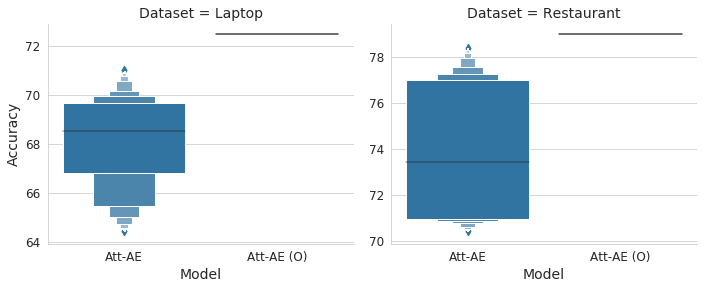
\includegraphics[scale=0.5]{images/augmentation/methods_performance/Inter_Target/inter_target_reproducability.png}
    \caption{Distribution of eight scores and the line represents the mean value, for the original model this line represents their only reported score. Model name with a \textit{(O)} represents the score reported in the original models paper.}
    \label{fig:aug_inter_target_reproducability}
\end{figure}

Figure \ref{fig:aug_overall_inter_target_scores.png} presents the overall results across the different metrics for the inter target encoding models. For easier comparison, figure \ref{fig:aug_overall_difference_inter_target_scores} reports the metric differences between the inter target encoding models and their respective baseline. As can be seen the results are either no better or worse in the majority of cases, only for the \textit{TDLSTM} model for the \textit{STAC 1} metric on the Election dataset are the results better as the standard deviation bars are greater than zero. This shows without performing any statistical tests that, in general, target aware models are not any better than their baseline models. 

\begin{figure}[!h]
    \centering
    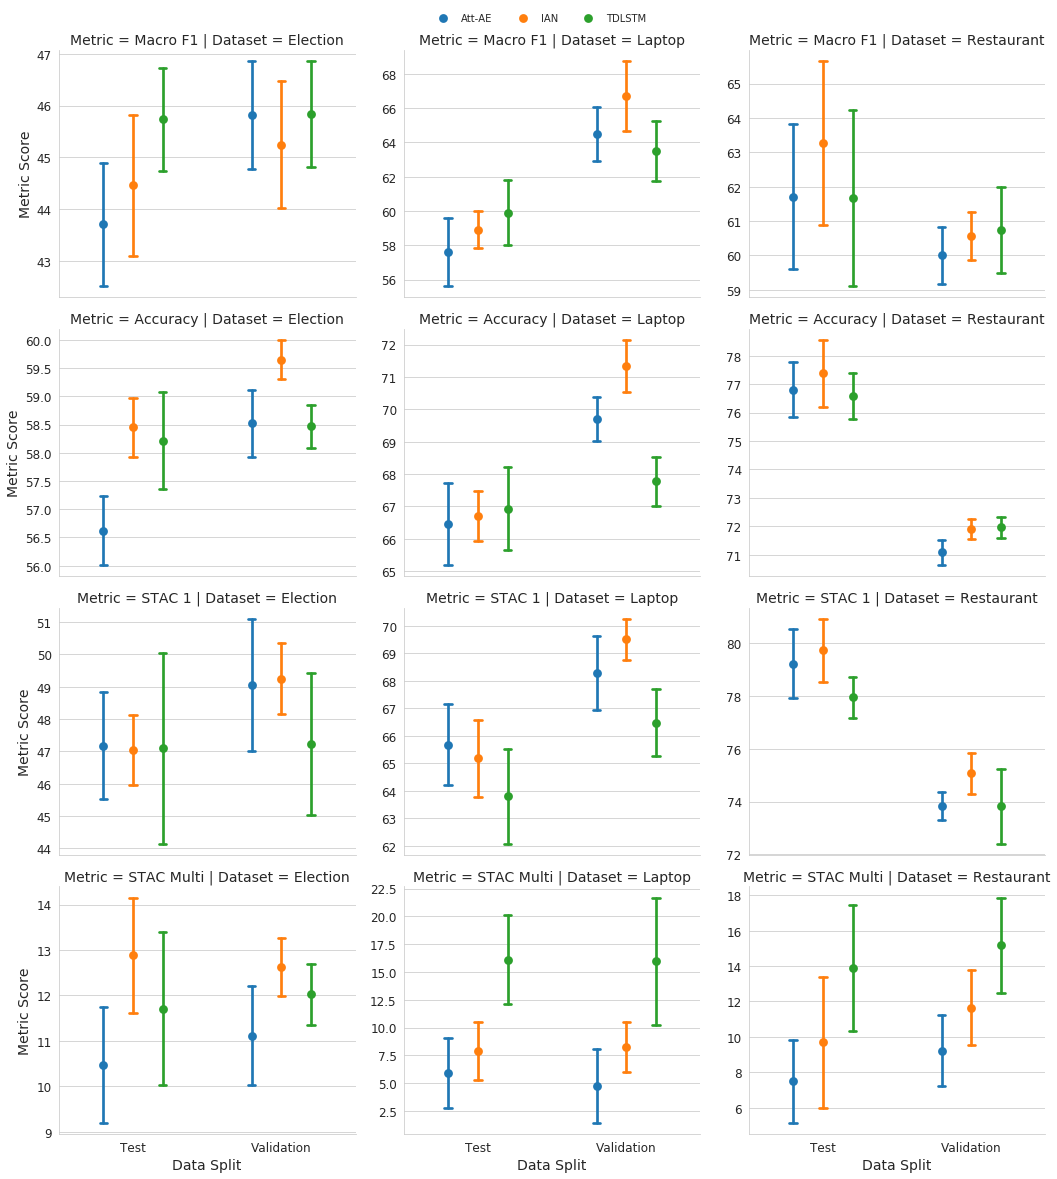
\includegraphics[scale=0.3]{images/augmentation/methods_performance/Inter_Target/overall_inter_target_scores.png}
    \caption{Each plot represents the three target aware enhanced models metric score on the test and validation splits. Columns represent different datasets, rows different metrics.}
    \label{fig:aug_overall_inter_target_scores.png}
\end{figure}
\begin{figure}[!h]
    \centering
    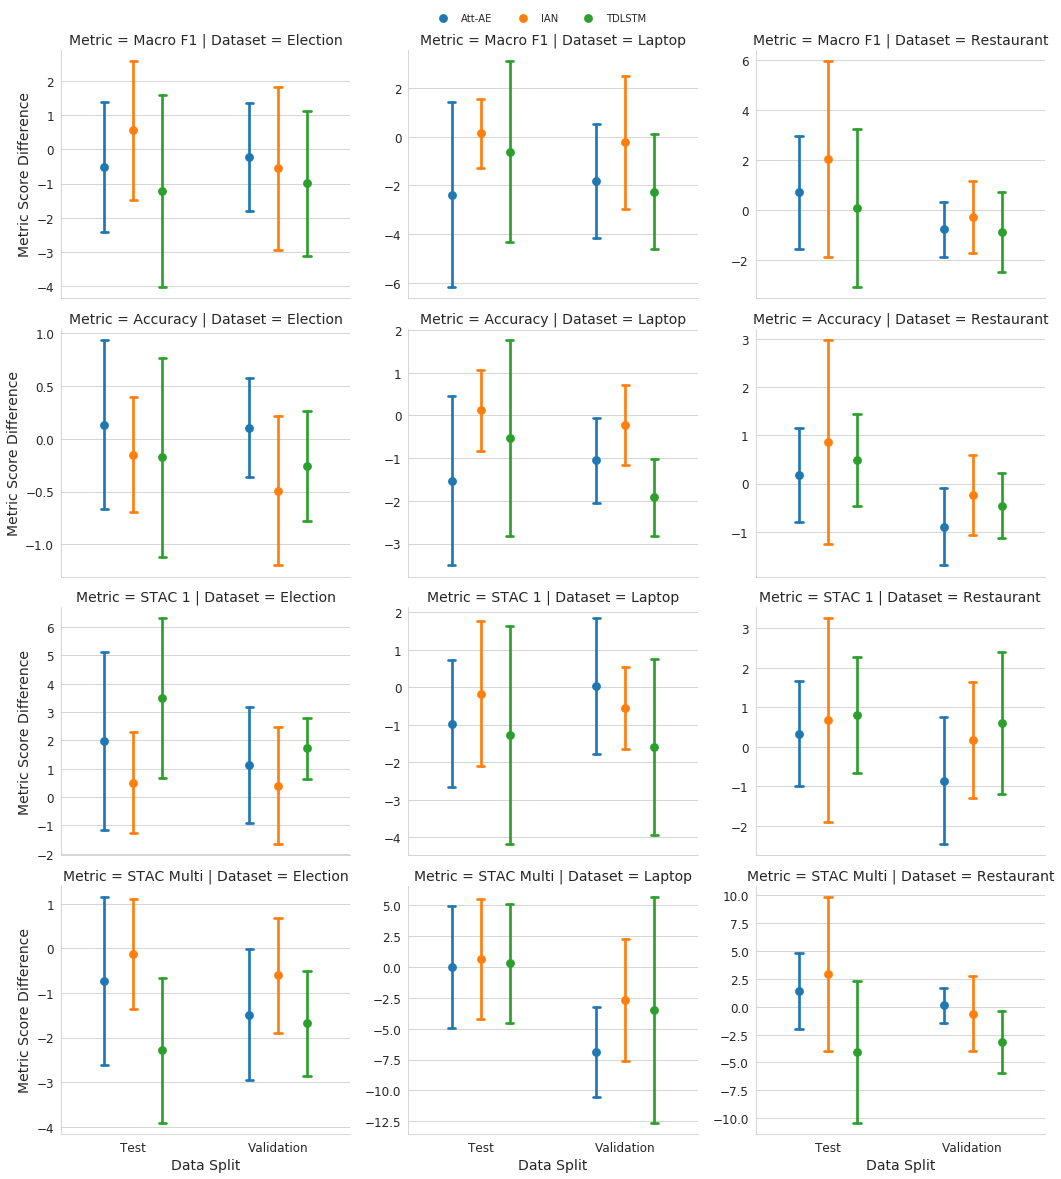
\includegraphics[scale=0.3]{images/augmentation/methods_performance/Inter_Target/overall_difference_inter_target_scores.png}
    \caption{Each plot represents the differences between the target aware and the baseline models for the relevant metric score on the test and validation splits. Columns represent different datasets, rows different metrics.}
    \label{fig:aug_overall_difference_inter_target_scores}
\end{figure}

Thus the heatmaps in figures \ref{fig:aug_dataset_sig_scores_inter_target} and \ref{fig:aug_combined_sig_scores_inter_target} show for the left (right) column the number of target aware (baseline) models that are statistically significantly better than their baseline (target aware) models, where the former is not corrected for multiple significance tests whereas the later is using
Bonferroni and is aggregated across datasets. As can be seen the only significant metric difference for the target aware models is on the \textit{STAC 1} metric for the Election dataset, of which when corrected with Bonferroni does not exist. On the other hand the baseline models appear to be better on the accuracy and \textit{STAC Multi} metric across both test and validation splits. This may suggest that for the Election dataset at least that the target aware models are somewhat overfitting to the most frequent sentiment more as they improve the results on the \textit{STAC 1} metric while becoming worse on the \textit{STAC Multi} metric. This would seem intuitive as the model could take advantage of knowing roughly the sentiment of all of the other targets within the sentence due to it's target awareness, and thus take the most likely overall sentiment. However as the number of target aware models that are significantly worse (better) while taking into account multiple tests is low (none) and none for the validation and test splits the assumption of sentiment overfitting cannot be empirically shown. This does show that target aware models from these metrics are not any better and in some cases worse than their baseline equivalent.

\begin{figure}[!h]
    \centering
    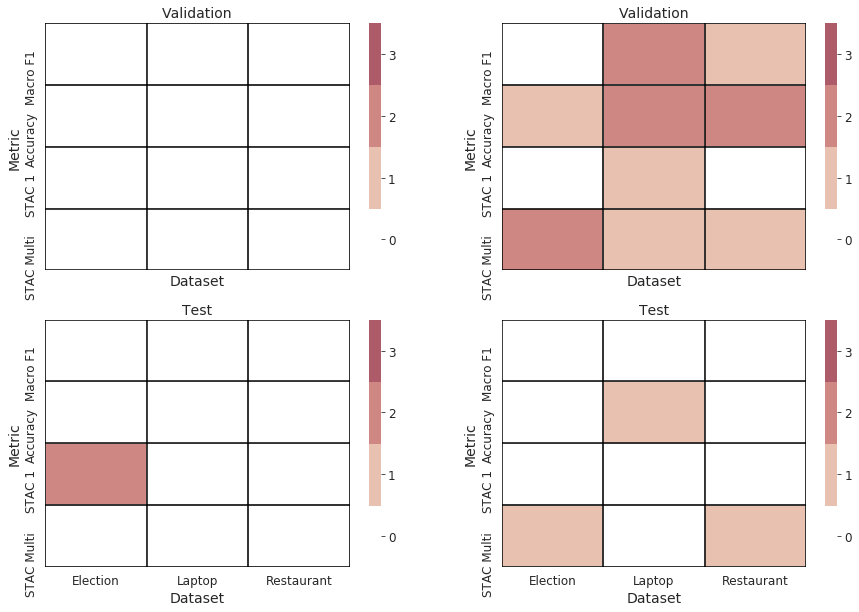
\includegraphics[scale=0.35]{images/augmentation/methods_performance/Inter_Target/dataset_sig_scores_inter_target.png}
    \caption{The left (right) hand side heatmaps represent the number of target aware (baseline) models that are statistically significantly better than their baseline (target aware) equivalents at the 95\% confidence level.}
    \label{fig:aug_dataset_sig_scores_inter_target}
\end{figure}
\begin{figure}[!h]
    \centering
    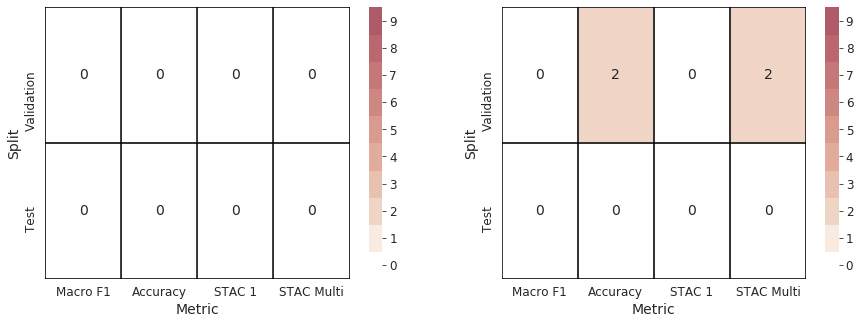
\includegraphics[scale=0.35]{images/augmentation/methods_performance/Inter_Target/combined_sig_scores_inter_target.png}
    \caption{The left (right) hand side heatmaps represent the number of target aware (baseline) models that are statistically significantly better than their baseline (target aware) equivalents across all datasets at the 95\% confidence level. Where the multiple hypothesis tests have been corrected using Bonferroni.}
    \label{fig:aug_combined_sig_scores_inter_target}
\end{figure}

Given these results strongly indicate the target aware models are no better, if not at times worse, than their baseline equivalents, the results comparing target aware to the baseline models across \textit{DS} and \textit{TSR} error splits are shown in figures \ref{fig:aug_inter_target_split_dataset_heatmaps} and \ref{fig:aug_inter_target_split_combined_heatmap} \footnote{The accuracy results for each subset for the test (validation) split are shown in figure \ref{fig:aug_inter_target_encoding_split_overall_test} (\ref{fig:aug_inter_target_encoding_split_overall_validation}). The accuracy difference between the target aware and their associated baseline models are in figures \ref{fig:aug_inter_target_encoding_split_overall_diff_test} and \ref{fig:aug_inter_target_encoding_split_overall_diff_validation} for the test and validation split respectively. These results are within the appendix as they do not show any additional information that the heatmaps in figures do not represent better. They are also within the thesis itself for reproducibility reasons.}. These heatmaps \ref{fig:aug_inter_target_split_dataset_heatmaps} and \ref{fig:aug_inter_target_split_combined_heatmap} show once again that the target aware models are not any better than their baseline equivalents on any subset of any split of any dataset consistently across data splits. Furthermore even though the baseline models are significantly better and consistently better for some subsets of splits as shown in figure \ref{fig:aug_inter_target_split_dataset_heatmaps} when corrected for multiple testing they are not, as shown in figure \ref{fig:aug_inter_target_split_combined_heatmap}. Thus this shows once again the target aware models are no better if not worse in some cases than their baseline equivalents.

\begin{figure}[!h]
    \centering
    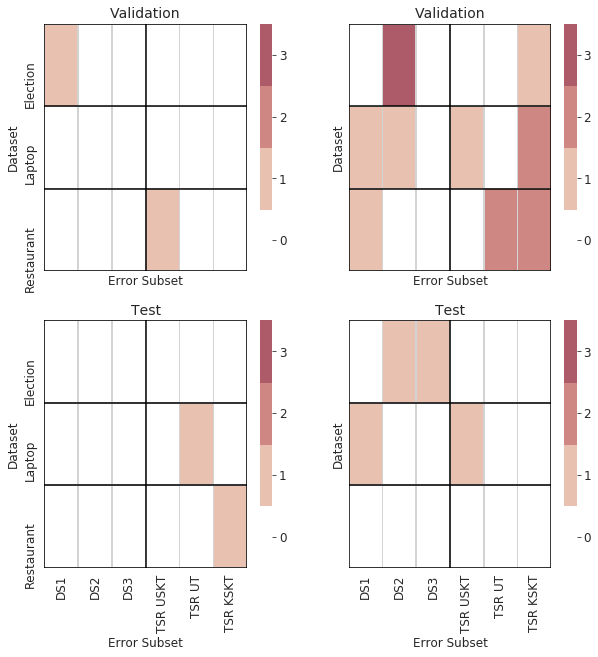
\includegraphics[scale=0.4]{images/augmentation/methods_performance/Inter_Target/inter_target_split_dataset_heatmaps.png}
    \caption{The left (right) hand side heatmaps represent the number of target aware (baseline) models that are statistically significantly better than their baseline (target aware) equivalents at the 95\% confidence level.}
    \label{fig:aug_inter_target_split_dataset_heatmaps}
\end{figure}
\begin{figure}[!h]
    \centering
    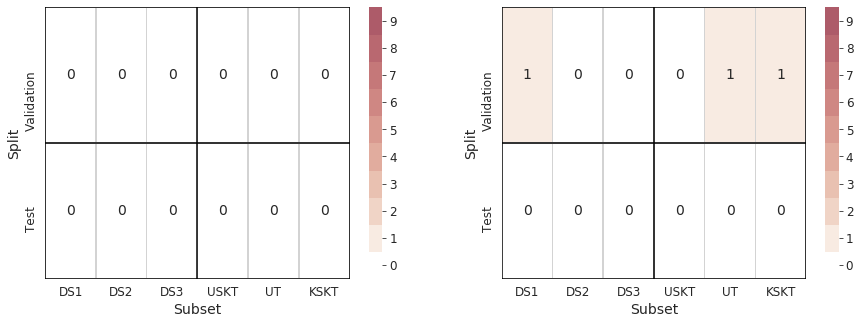
\includegraphics[scale=0.35]{images/augmentation/methods_performance/Inter_Target/inter_target_split_combined_heatmap.png}
    \caption{The left (right) hand side heatmaps represent the number of target aware (baseline) models that are statistically significantly better than their baseline (target aware) equivalents across all datasets at the 95\% confidence level. Where the multiple hypothesis tests have been corrected using Bonferroni.}
    \label{fig:aug_inter_target_split_combined_heatmap}
\end{figure}

\subsection{Conclusion}
To conclude, even though the previous works that incorporated some form of target awareness into their models have shown improvements over their own baseline models \citep{zhao2019modeling, fan-etal-2018-multi}, this has not been shown here. Furthermore it has been shown that on some datasets and some baseline models that they are significantly better than their target aware version. This negative result showing that unlike the previous work here it has been shown that the target aware models are no better than their baseline models could be due to none of the previous works performing rigorous testing of their methods. In all of the previous works none of them perform statistical significant testing nor do they take into account the random seed problem \citep{reimers-gurevych-2017-reporting} which has been shown significant in chapter \ref{chapter:reproducibility} for NN TDSA methods. In comparison this work takes both the significance testing and random seeds into account. Even though it was shown that the \textit{Att-AE} model could not reproduce the results from the original paper \citep{hazarika-etal-2018-modeling}, it can be concluded here that at least for \citet{hazarika-etal-2018-modeling} inter target encoding method it does not perform any better than not using it. Even though it is stating that opposite of  \citet{hazarika-etal-2018-modeling}, the results here are more rigorously tested and on more models and datasets.

\section[Contextualised Word Representations (CWR)]{Contextualised Word Representations (CWR)\footnote{All graphs within this section have been generated through the following notebook \url{https://github.com/apmoore1/tdsa_comparisons/blob/master/analysis/CWR.ipynb}.}}
\label{section:aug_cwr}
\subsection{Introduction}
\label{section:aug_cwr_intro}
% (Looks at point 2 and 3 from the introduction)

%In this section, we are going to look at three different types of Neural Network (NN) systems:
%\begin{enumerate}
%    \item TDLSTM -- A RNN based NN that encodes the target by ensuring the target word(s) are always the last word(s) fed to the RNN from the context. Thus a position based method where the position is encoded through the NN architecture.
%    \item IAN -- Encodes the target into the context via attention.
%    \item InterAE -- Encodes the target into the context by fusing the context and target representations to create a target-context sequence. It further encodes the target into this new target-context sequence by applying attention using the target representation. Then models the other targets within the same context by using an RNN.  
%\end{enumerate}
%Thus to summarise the differences in these TDSA methods; TDLSTM encodes the position of targets through its architecture, IAN encodes the target into the context via attention, and InterAE encodes the target similar to IAN but further models other targets within the same context. Thus using three different types of methods and three different datasets this will ensure that the experimental results and findings to be robust and generalisable. In this subsection the thesis will: 
%\begin{enumerate}
%    \item Review the state of CWR within TDSA and the findings that already exist within the literature. 
%    \item Confirm prior works findings on CWR improving results over non-CWR, as well as the benefits of pre-training CWR.
%    \item How CWR improve TDSA model through novel error analysis.
%\end{enumerate}
  
%\begin{enumerate}
%    \item Are general CWR significantly better than Glove (non-CWR) representations.
%    \item Are domain specific CWR significantly better than general CWR.
%\end{enumerate}
%Furthermore given the better CWR the thesis will explore the differences between CWR and non-CWR with respect to the different splits stated in the error analysis section \ref{section:aug_error_analysis}. Thus showing what gains CWR bring to TDSA and more importantly what is still difficult to classify within TDSA.

%As stated in the introductory section of this chapter \ref{section:aug_introduction}, the three datasets that are used throughout this chapter are the Election, Laptop and Restaurant datasets. However unlike the error analysis section \ref{section:aug_error_analysis}, the standard training split for each of the datasets will be further randomly split into a new training and an additional validation split, and the size of these splits can be seen in table \ref{table:aug_cwr_split_breakdown}. The validation set is required so that the early stopping can be used for all of the NN methods. Furthermore, the validation set would usually be used for more hyper-parameter tuning e.g. finding the best learning rate etc. but due to compute time this is not the case. Instead we selected the most common hyper-parameters from the literature as detailed in table \ref{table:aug_cwr_default_hyperparameters}, it will be stated explicitly within this chapter if these hyperparameters are not used. Lastly all results reported in this section will be results on the test set and all validation results will be reported in the appendix for reproducibility reasons \citep{dodge-etal-2019-show}. However if there is a large difference between the validation and test results this will be mentioned explicitly in this section.

%\begin{table}[ht!]
%    \centering
%    \begin{tabular}{|c|c|c|c|c|}
\hline
        & \multicolumn{4}{c|}{Data Split} \\
\hline
Dataset &          Train &     Validation &           Test &  Total \\
\hline
Election   &  6811 (57.24\%) &  2547 (21.41\%) &  2541 (21.35\%) &  11899 \\
\hline
Laptop     &  1661 (56.29\%) &   652 (22.09\%) &   638 (21.62\%) &   2951 \\
\hline
Restaurant &  2490 (52.73\%) &  1112 (23.55\%) &  1120 (23.72\%) &   4722 \\
\hline
\end{tabular}
%    \caption{Number of samples.}
%    \label{table:aug_cwr_split_breakdown}
%\end{table}

%Due to the splitting of the training dataset, the error analysis split statistics in section \ref{section:aug_error_analysis} will not be identical for the global error splits (\textit{n-shot} and \textit{TRS}) between the train/test and train/validation as they rely on a comparison of train and validation/test. Even though they will not be identical they are relatively similar as shown by table \ref{table:aug_cwr_global_error_diff}. Furthermore as the local splits ($DS_i$, \textit{NT}, and \textit{TSSR}) are only reported for the test set, table \ref{table:aug_cwr_local_error_diff} shows them for the validation and test set showing that they are again relatively similar, thus results should be comparable between validation and test sets.  


The majority of TDSA work so far has only used the standard 840 billion token 300 dimensional GloVe vectors \citep{pennington-etal-2014-glove} to initialise word representation within the NN \citep{tang-etal-2016-aspect,tang-etal-2019-progressive}. These non-CWR word vectors in effect transfer semantic and syntactic knowledge of words from the semi-supervised task they were trained from \citep{mikolov2013efficient}. Due to this transferring of knowledge they have been shown to help in multiple NLP settings such as Semantic Role Labelling \citep{collobert2008unified}, Named Entity Recognition, Chunking \citep{turian-etal-2010-word}, and text classification \citep{kim-2014-convolutional}. The word vectors are normally the embedding layer (the first layer) of the NN that is usually trained with a Language Model (LM) type of objective. Thus the data they train from does not require any human annotation. Due to the word vectors coming from this embedding layer the vectors themselves are not contextualised as the NN at this point has not seen any of the other words within the context/text. Therefore the main drawback of non-CWR is that they suffer from word ambiguity \citep{camacho2018word}. 

To overcome this, CWR have been devised which are still trained on a LM objective, but instead of using the embedding layer they either use the second to last layer of the NN \citep{peters-etal-2017-semi}, or a weighted combination of each layers weights which has been shown to be more effective \citep{peters-etal-2018-deep}. These CWR have been shown to outperform non-CWR across a spectrum of NLP tasks by a large margin \citep{liu-etal-2019-linguistic}. The CWR work that has been stated are used in a \textit{feature based} approach where the CWR are fed to a task specific architecture. However, work has also been focused on an alternative approach \textit{fine-tuning} where normally the last layer of the LM NN is replaced with a new task specific layer, and then the whole NN is tuned to the new task \citep{radford2018improving, howard-ruder-2018-universal}. This approach has become very popular since the arrival of BERT \citep{devlin-etal-2019-bert}, due to its impressive performance across multiple tasks compared to other State Of The Art (SOTA) approaches, and its accessibility through the release of its code base\footnote{\url{https://github.com/google-research/bert}}. 

For the interested reader on CWR, there are many different CWR each with subtle differences. These differences are normally based around their learning objective e.g. Bi-LM \citep{peters-etal-2018-deep}, masked LM \citep{devlin-etal-2019-bert}, etc, how they are trained e.g. discriminative fine-tuning \citep{howard-ruder-2018-universal}, model design choices \citep{liu2019roberta}, distillation \citep{tsai-etal-2019-small}, etc if they are multi-lingual \citep{conneau2019cross}, multi task learning with supervised objectives \citep{liu-etal-2019-multi}, for a whole list of papers on CWR see the following GitHub list\footnote{\url{https://github.com/thunlp/PLMpapers}}.

As stated in the introduction section \ref{section_case_intro}, previous works have already started to use CWR within TDSA, of which a comprehensive list of these works and metadata details can be seen in table \ref{table:aug_cwr_tdsa_cwr_methods_overview}\footnote{This is most likely already out of date due to the speed that new publications are coming out, and the fact that CWR produce the SOTA results.}. The table clearly shows that a lot of the prior works have tried different architectures: Task Specific Architecture (TSA) and non-TSA\footnote{non-TSA is defined as adding a linear layer on top of the CWR class vector in the case of the BERT model (which is the only CWR model used in prior work).}, fine-tuning or feature based, and pre-training the CWR and not. From this prior work some general insights can be drawn, which will be discussed below.

Pre-training in this thesis is defined as the process of fine-tuning the LM NN that the CWR come from with a separate task and dataset before using the LM NN on the final task, which here is TDSA. A concrete example of pre-training from table \ref{table:aug_cwr_tdsa_cwr_methods_overview}, is pre-training to Yelp and/or Amazon datasets by using an LM objective to fine-tune the BERT\textsubscript{b} LM NN to these dataset, thus making the BERT\textsubscript{b} model more domain specific. Generally one would expect pre-training to improve results as it adapts the CWR to the domain, and this is what both \citet{rietzler2019adapt} and \citet{xu-etal-2019-bert} found. However considering both works use the same pre-training datasets and technique, as well as same CWR and model architecture there is a 2-3\% difference in results. This is most likely due to the lack of pre-training that \citet{xu-etal-2019-bert}\footnote{Used around 1 and 2 million sentences for Laptop and Restaurant domain respectively. This was calculated by multiplying the batch size (16) by the number of training steps.} did not perform, as \citet{rietzler2019adapt} showed that at least 10 million sentences\footnote{These do not have to be the same sentences, as they had 1 million `unique' sentences and 10 million sentence comes from training the model for 10 epochs.} are required before any improvements can be seen for the Laptop domain.

Another insight that can be drawn from the works that use TSAs \citep{zeng2019lcf,zhao2019modeling,song2019attentional,huang-carley-2019-syntax, jiang-etal-2019-challenge} is that using a CWR instead of a non-CWR is always better. This finding is more interesting for the works that do not fine-tune the CWR \citep{zhao2019modeling, huang-carley-2019-syntax} as it shows that by using CWR alone, and not more parameters, results improve over using non-CWR. Furthermore \citet{song2019attentional}, \citet{jiang-etal-2019-challenge}, and \citet{huang-carley-2019-syntax} all found that using a TSA with CWR in a feature based or fine-tuning approach to be better than fine tuning the CWR model with no TSA.

Lastly shown in table \ref{table:aug_cwr_tdsa_non_cwr_methods_overview} are the best performing non-CWR methods\footnote{In both cases they are using GloVe vectors and have a TSA.}, of which these are a lot worse in performance compared to any of the CWR methods within table \ref{table:aug_cwr_tdsa_cwr_methods_overview}.

\begin{landscape}% Landscape page
        %\centering
        \begin{table}
\centering
\begin{tabular}{|c|c|c|c|c|c|c|}
\hline
Authors & Laptop (\%) & Restaurant (\%) & Fine Tuned &  CWR Model & Pre-Trained & TSA \\
\hline
\cite{rietzler2019adapt}   & 80.23 &  \textbf{87.89} &  Yes &  BERT\textsubscript{b} & Yelp, Amazon & No \\
\hline
\cite{zeng2019lcf}   & \textbf{82.45} &  87.14 &  Yes &  BERT\textsubscript{b} & No & Yes \\
\hline
\cite{jiang-etal-2019-challenge}   & - &  85.93 &  Yes &  BERT\textsubscript{b} & No & Yes \\
\hline
\cite{xu-etal-2019-bert}   & 78.07 & 84.95  &  Yes &  BERT\textsubscript{b} & Yelp , Amazon, SQuAD & No \\
\hline
\cite{zhao2019modeling}   & 81.35 &  83.57 &  No &  BERT\textsubscript{b} & No & Yes \\
\hline
\cite{song2019attentional}   & 79.93 &  83.12 &  Yes &  BERT\textsubscript{b} & No & Yes \\
\hline
\cite{huang-carley-2019-syntax}   & 80.1 &  83.0 &  No &  BERT\textsubscript{l} & No & Yes \\
\hline
\multicolumn{7}{|c|}{Bert\textsubscript{b}=BERT base model, Bert\textsubscript{l}=BERT large model \citep{devlin-etal-2019-bert}} \\
\multicolumn{7}{|c|}{TSA=Task Specific Architecture} \\
\hline
\end{tabular}
\caption{Overview of TDSA methods that use CWR}
\label{table:aug_cwr_tdsa_cwr_methods_overview}
\end{table}
\end{landscape}

\begin{table}[!h]
    \centering
    \begin{tabular}{|c|c|c|}
\hline
Authors & Laptop (\%) & Restaurant (\%)\\
\hline
\cite{zhao2019modeling}   & 75.55 &  \textbf{82.95}\\
\hline
\cite{zeng2019lcf}   & \textbf{76.02} &  82.5\\
\hline
\end{tabular}
    \caption{Top performing non-CWR TDSA methods}
    \label{table:aug_cwr_tdsa_non_cwr_methods_overview}
\end{table}

Thus to summarise from this prior work, we can determine that:
\begin{enumerate}
    \item Pre-training is always useful but to be fully utilised it requires fitting on large amounts of pre-training data.
    \item Using a TSA with CWR is better than using no TSA with CWR.
    \item Using CWR is always better than non-CWR.
\end{enumerate}

%Another interesting difference in the prior works is fine-tuning and Task Specific Architecture (TSA), where no TSA means that only a linear layer is added on top of the CWR model. It would appear based on \citet{zeng2019lcf} that fine-tuning is always better if you have a TSA. However this would contradict the results from \citet{song2019attentional}, which showed for one dataset out of the three evaluated on that the original BERT model fine-tuned was better than there TSA with BERT fine-tuned. Thus this shows some discrepancies between works and that certain TSA are better than others at utilising CWR. Furthermore it has been shown for NER that fine-tuning a BERT type model with a large TSA on top is not optimal \citep{peters-etal-2019-tune}. 

%These works mainly use a non-task specific BERT model \citep{devlin-etal-2019-bert}, where they use a st

The CWR that will be used to investigate the effect it has on the TDSA and text classification methods in this thesis is the ELMo transformer (ET)\footnote{The base ET model can be found here \url{https://allennlp.org/elmo} named as the `Transformer ELMo' model.} as it is quicker for both training and inference than the standard LSTM ELMo, and generally better than a Gated CNN version \citep{peters-etal-2018-dissecting}. Furthermore this is used in the \textit{feature based} manner with a weighted combination of it each layers weights. \textit{Feature based} was chosen over \textit{fine-tuning} as \textit{fine-tuning} adds a large number of parameters to the task specific model, which would therefore mean that we are testing not just CWR but also the affect of adding more parameters. The effect of adding more parameters is thus undesirable and not needed, hence a \textit{feature based} approach was chosen. Furthermore ET was chosen over BERT due to practicalities of training these models at the time of experimentation. Lastly the point of these experiments is to test the differences between CWR and non-CWR rather than differences in CWR for TDSA. As it has been shown in the prior work that domain specific CWR out perform non-domain specific, the ET model is pre-trained using an LM task for each domain Laptop, Restaurant and Election. For the Laptop dataset the ET model is pre-trained on the Amazon electronics reviews dataset\footnote{Can be found here \url{http://jmcauley.ucsd.edu/data/amazon/}} \citep{mcauley2015image}, where the ET model is trained on 28,742,985 in domain sentences. The Restaurant dataset uses the 2019 Yelp dataset\footnote{\url{https://www.yelp.com/dataset}} where the ET model is trained on 27,286,698 in domain sentences. Finally the Election dataset unlike the others trains the ET model from scratch on 9,903,000 in domain tweets\footnote{These tweets were collected by scraping Tweets that originate from the current MPs of the time.}. All of the detailed pre-processing, analysis and training of these domain sepcific ET models can be found here \url{https://github.com/apmoore1/language-model}. As \citet{rietzler2019adapt} found that at least 10 million pre-training sentences are required before the CWR models perform any better than their non-domain specific CWR, furthermore the performance of their models saturate after 17 million sentences. This advice from \citet{rietzler2019adapt} has been followed for the Laptop and Restaurant ET models but not the Election ET model. Within the experiment section considering non of the prior work investigated what affect the CWR had on TDSA and text classification methods other than overall Accuracy and macro F1, this will be explored through the recommended metrics and error splits. 

\subsection{Experiments}
To fully report the results figure \ref{fig:aug_overall_cwr_results} shows the different metric scores the CWR TDSA and text classification (\textit{CNN}) models scored on all datasets. The more informative is figure \ref{fig:aug_overall_diff_cwr} which compares the metric scores of the CWR and their respective baseline models. From this figure it can be seen that all of the TDSA models perform better on almost every metric. The \textit{STAC 1} metric on the Election dataset some of the TDSA models perform worse/no better, which may suggest the models are becoming better at the target sentiment relationship modelling and overfitting less to the most frequent sentiment in the sentence as they improve on the \textit{STAC Multi} metric. Also some of the TDSA models perform worse/no better on the \textit{STAC Multi} metric on the Laptop and Restaurant dataset but perform much better on the \textit{STAC 1} metric suggesting the models are overfitting to the most frequent sentiment in the sentence. This initial analysis suggests to some extent that the CWR increase the performance of the TDSA model by exploiting the artefacts of the datasets. This is shown through the fact that the datasets that contain the least number of $DS_2$ and $DS_3$ sentences, Laptop and Restaurant, the CWR TDSA models perform a lot better compared to their baseline on the \textit{STAC 1} metric, but not the \textit{STAC Multi}. Where as the Election dataset that contains more sentences of $DS_2$ and $DS_3$ combined than $DS_1$, the CWR models perform better compared to their baseline on the \textit{STAC Multi} than the \textit{STAC 1} in general. 

\begin{figure}[!h]
    \centering
    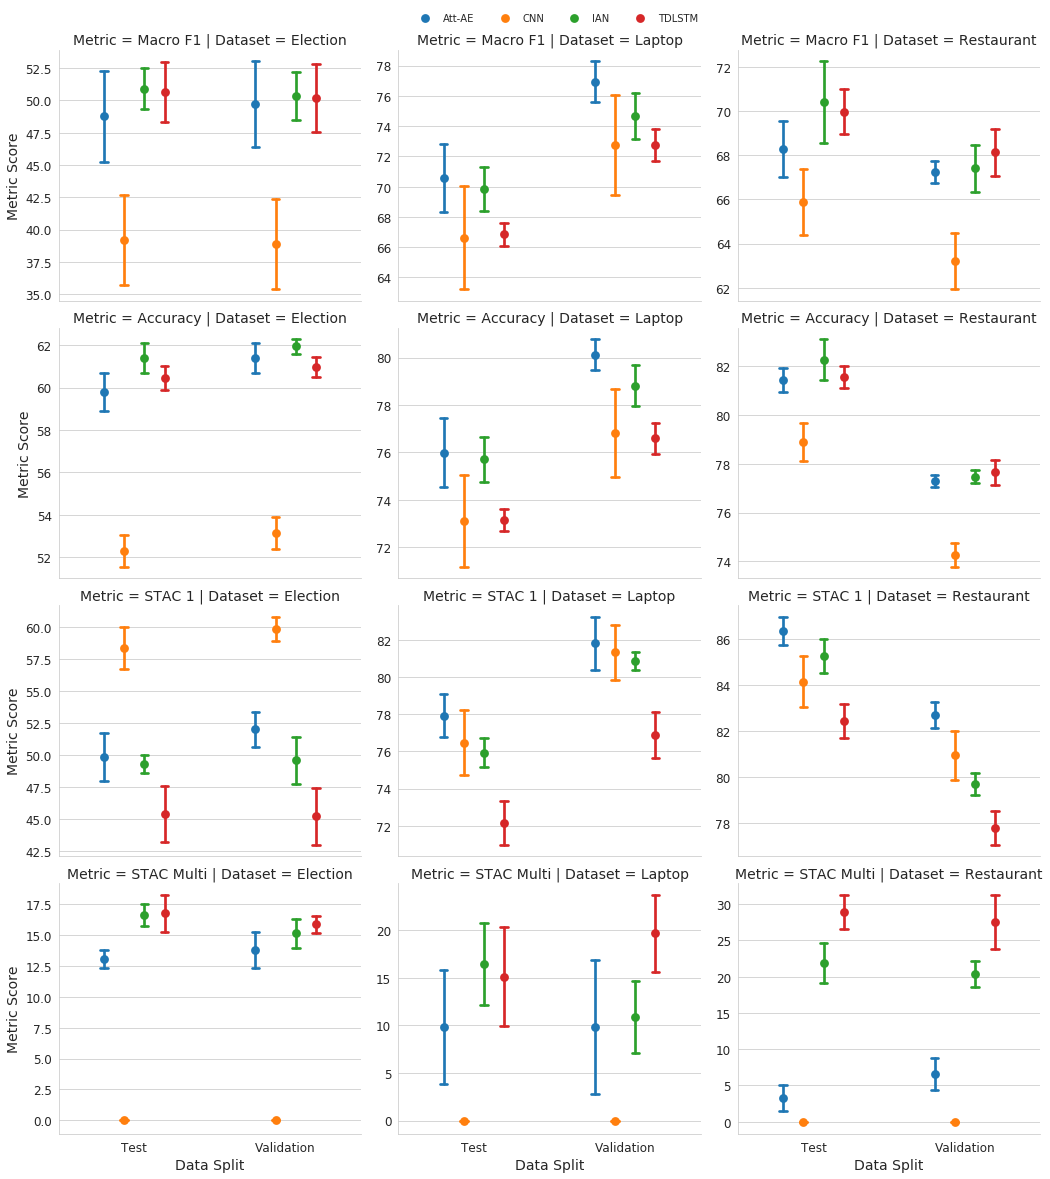
\includegraphics[scale=0.3]{images/augmentation/methods_performance/CWR/overall_cwr_results.png}
    \caption{Each plot represents the CWR models metric score on the test and validation splits. Columns represent different datasets, rows different metrics.}
    \label{fig:aug_overall_cwr_results}
\end{figure}

\begin{figure}[!h]
    \centering
    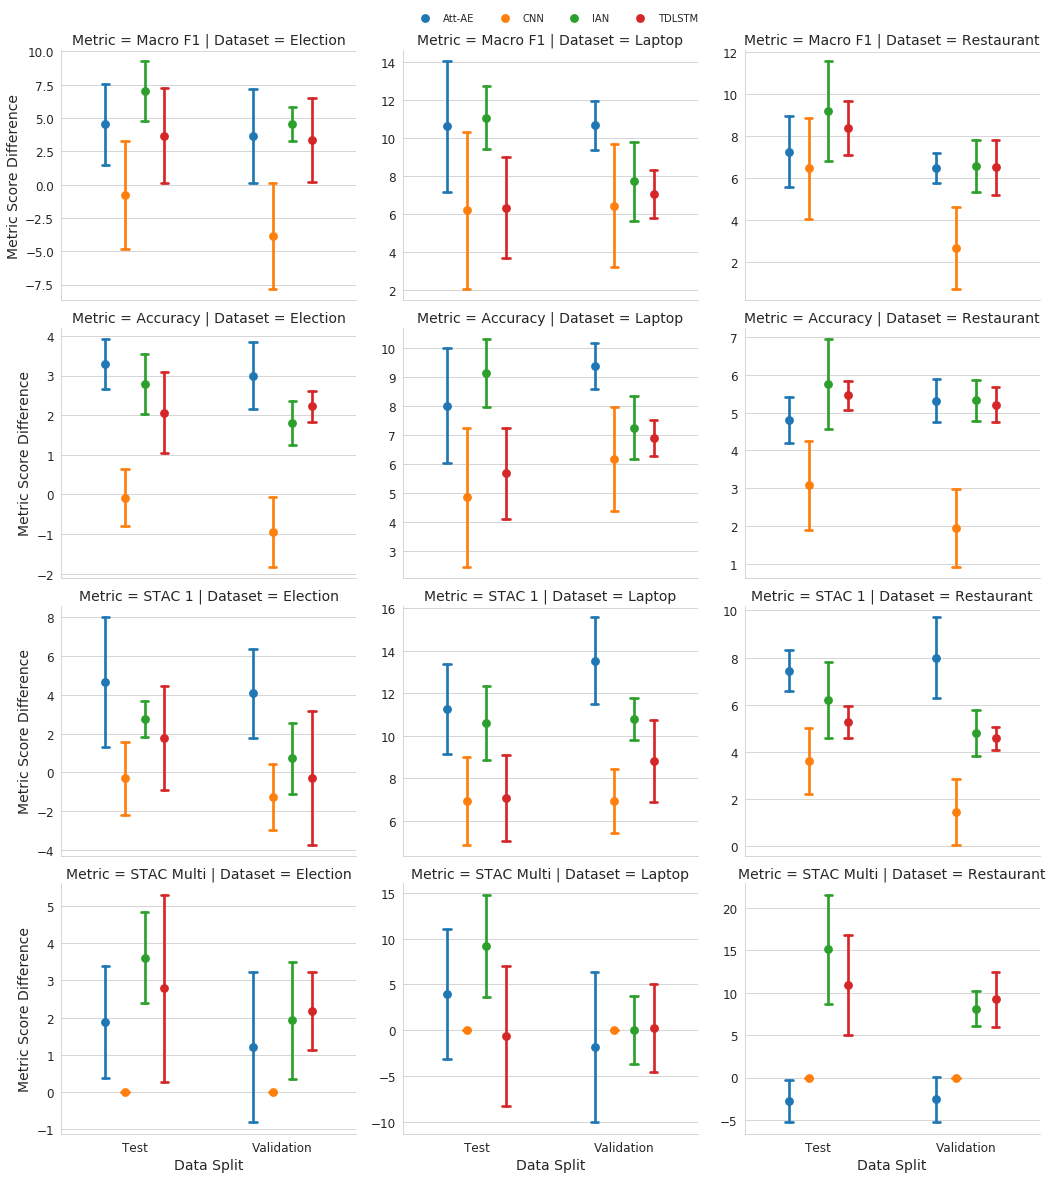
\includegraphics[scale=0.3]{images/augmentation/methods_performance/CWR/overall_diff_cwr.png}
    \caption{Each plot represents the differences between the CWR and the baseline models for the relevant metric score on the test and validation splits. Columns represent different datasets, rows different metrics.}
    \label{fig:aug_overall_diff_cwr}
\end{figure}

To investigate this further the heatmaps in figure \ref{fig:aug_cwr_dataset_metric_sig} and \ref{fig:aug_cwr_sig_metric}\footnote{This heatmap does not show the number of baseline models that are significantly better than their CWR model as none were.} show the number of TDSA only CWR models that are statistically significantly better than their baseline, where the former is not correct for multiple significance tests where as the later is using Bonferroni and is aggregated across datasets. It can be seen that for the accuracy metric the CWR improve over the baseline significantly. Macro F1 when corrected for multiple tests it is not shown as significant as seen in figure \ref{fig:aug_cwr_sig_metric}. In general and as stated before the CWR models perform significantly better on the \textit{STAC Multi} for the Election dataset but for those that contain far fewer $DS_2$ and $DS_3$ samples this is not true. The \textit{STAC 1} metric is similar to the accuracy in that in almost all cases the CWR are significantly better than their baselines. These significant test some what agree with the initial analysis that the CWR are exploiting the artefacts of the datasets, as they perform generally no better on the \textit{STAC Multi} metric for datasets that contain far fewer $DS_2$ and $DS_3$ samples (Laptop and Restaurant).

\begin{figure}[!h]
    \centering
    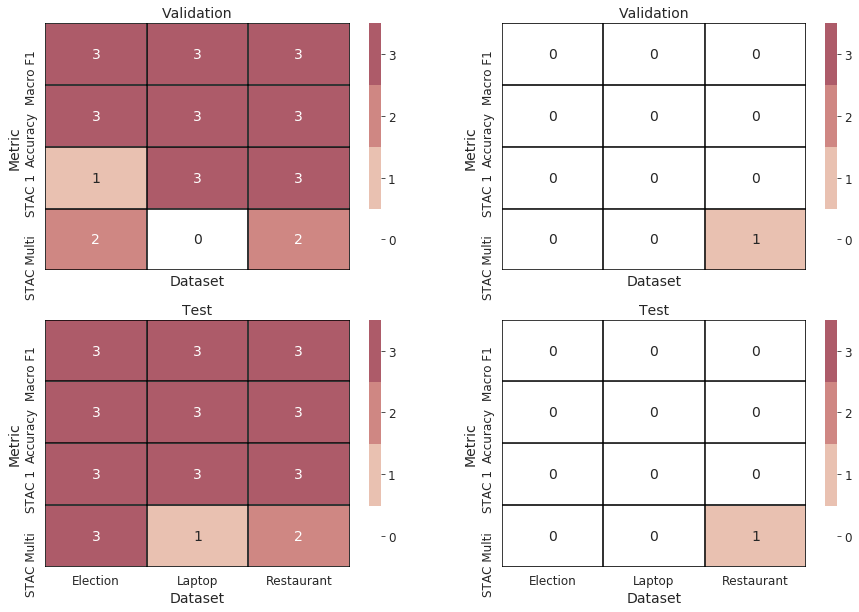
\includegraphics[scale=0.4]{images/augmentation/methods_performance/CWR/cwr_dataset_metric_sig.png}
    \caption{The left (right) hand side heatmaps represent the number of CWR (baseline) models that are statistically significantly better than their baseline (CWR) equivalents at the 95\% confidence level.}
    \label{fig:aug_cwr_dataset_metric_sig}
\end{figure}

\begin{figure}[!h]
    \centering
    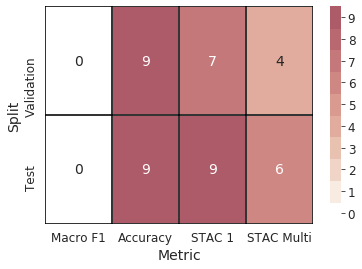
\includegraphics[scale=0.4]{images/augmentation/methods_performance/CWR/cwr_sig_metric.png}
    \caption{The number of CWR models that are statistically significantly better than their baseline equivalents across all datasets at the 95\% confidence level. Where the multiple hypothesis tests have been corrected using Bonferroni.}
    \label{fig:aug_cwr_sig_metric}
\end{figure}

To further investigate whether this initial analysis is true the \textit{DS} error split significance heatmaps can be seen in figures \ref{fig:aug_cwr_dataset_sig_error_splits} and \ref{fig:aug_cwr_combined_sig_error_splits}. Also within those heatmaps are the \textit{TSR} error analysis results, which can be used to study if the CWR improve zero shot target and sentiment relation prediction through the \textit{UT} and \textit{USKT} subsets respectively. The results from the \textit{DS} error splits some what confirm the initial analysis as the laptop validation results for the $DS_2$ subset have no significantly better CWR models. Furthermore out of the nine possible model and dataset combinations only six and five models are significantly better than their baseline for the $DS_2$ subset on the test and validation data splits respectively. This in comparison to almost all CWR models significantly better on the $DS_1$ subset. In comparison to any of the other enhancements this is the first time that the \textit{UT} and \textit{USKT} subsets have improved significantly. This suggests that contextualising the target representations greatly improves the generalisation of them to new targets that are most likely similar to seen targets.

\begin{figure}[!h]
    \centering
    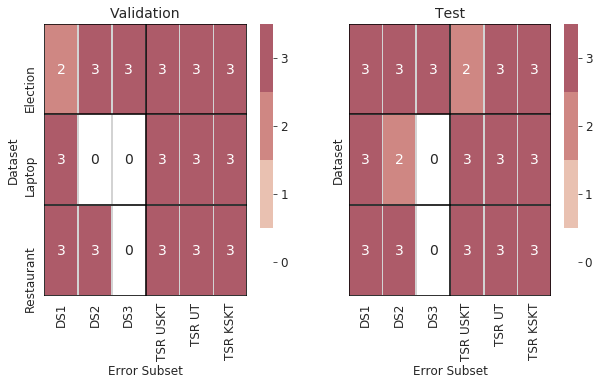
\includegraphics[scale=0.5]{images/augmentation/methods_performance/CWR/cwr_dataset_sig_error_splits.png}
    \caption{The left (right) hand side heatmaps represent the number of CWR (baseline) models that are statistically significantly better than their baseline (CWR) equivalents at the 95\% confidence level.}
    \label{fig:aug_cwr_dataset_sig_error_splits}
\end{figure}

\begin{figure}[!h]
    \centering
    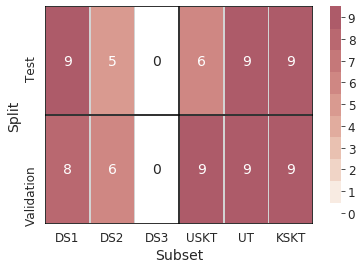
\includegraphics[scale=0.5]{images/augmentation/methods_performance/CWR/cwr_combined_sig_error_splits.png}
    \caption{The number of CWR models that are statistically significantly better than their baseline equivalents across all datasets at the 95\% confidence level. Where the multiple hypothesis tests have been corrected using Bonferroni.}
    \label{fig:aug_cwr_combined_sig_error_splits}
\end{figure}

\subsection{Conclusion}
To conclude, in accordance with the existing literature, it is found that through the general accuracy metric CWR improve TDSA methods significantly compared to using non-CWR (baseline). Unlike the previous work, much greater emphasis has been placed on finding for the first time how CWR improve TDSA models. It has been shown here that the CWR significantly improve the performance of samples that contain unknown targets (\textit{UT}) or unknown sentiment relationship (\textit{USKT}). Thus suggesting that CWR model will perform better in the real world or low resource setting where a lot of the targets or sentiment relationships are not known. It was also found that the macro F1 scores for the CWR are significantly better than their non-CWR but when correcting for multiple tests was not found to be true. The CWR would appear to only improve significantly for the \textit{STAC Multi} metric and $DS_2$ subsets when the dataset contains more $DS_2$ and $DS_3$ samples like the Election dataset, improving the target sentiment relationship modelling for those TDSA models. Where as the CWR would almost always improve the \textit{STAC 1} metric and accuracy on the $DS_1$ subset, this suggesting that in some cases the CWR maybe overfitting to the most frequent sentiment in the sentence. Lastly unlike the previous CWR works the overall accuracy results are somewhat lower. This could be due to the fact that a different CWR model was used, ET instead of BERT. Where BERT\textsubscript{b}, even though it contains a similar transformer architecture, it has 12 transformer layers compared to ET's 6. Even though the number of layers this may not be significant, it has been shown for cross lingual performance in Natural Language Inference to be of great importance \citep{wang2019cross} \footnote{See table 4. Depth in table 4 is the same as layers.}. 

\section{Conclusion}
%The research question that this chapter was attempting to answer is `How can TDSA methods be measured quantitatively?'. To investigate this, section \ref{section:aug_error_analysis} reviewed the prior work in error analysis splits within TDSA. From this literature review, several existing error splits were found \textit{DS} which measured target sentiment relationship modelling, \textit{NT} measuring target interaction, and \textit{n-shot} measuring generalisation to unknown targets. From this literature review, two novel error splits were created \textit{TSSR} that measured target sentiment overfitting to the most frequent sentiment in a sentence and \textit{TSR} measuring generalisation to unknown sentiment relationships and targets. These existing error splits were rigorously tested in section \ref{section:aug_baseline} across three TDSA methods and a text classification method to ensure they were measuring what was hypothesised. From this \textit{NT} error split was removed due to it not measuring target interaction but rather the sentiment factors \textit{DS}. \textit{TSSR} was dropped due to it not measuring target sentiment overfitting without a text classification model and the \textit{DS} split. Lastly the \textit{n-shot} split was removed as when the value of \textit{n} increased it was expected the accuracy should increase as well or at the least not drop, which was not always true. Thus the \textit{TSR} split which measured both unknown targets and sentiment relationships was recommended as a better replacement to \textit{n-shot}. The findings from reviewing the \textit{NT} split bring the recommendation that the only way to investigate target interaction is through an annotated corpus with this explicitly annotated. A novel TDSA metric is created \textit{STAC Multi} and \textit{STAC 1} which when used together can be used to evaluate sentiment overfitting to the most frequent sentiment in the sentence. Furthermore \textit{STAC Multi} metric can be seen as a coarse grained version of the \textit{DS} error split as they both measure target sentiment relationship modelling, but \textit{STAC Multi} cannot be influenced by sentiment overfitting to the most frequent sentiment in the sentence. Thus from section \ref{section:aug_baseline} the error splits have been reduced to those that match there hypothesises and a new novel metric has been created to over come short comings from the error splits. 

From these three investigations, the position encoding showed successfully that the original hypothesis that adding position information does improve target sentiment relationship modelling, due to the position model's significant improvements on the \textit{STAC Multi} metric and $DS_2$ subset. Negative results were found for the inter target encoding experiments as all results showed that the baseline models were no worse if not at times better than their inter target encoded enhanced models. Furthermore the original hypothesis that inter target encoding was supposed to improve the model target interaction could not be measured using any error split or metric. Lastly, testing on the CWR where the main hypothesis from the previous work was that the models generally improved as shown through either the accuracy or macro F1 score was confirmed in this thesis. Furthermore, the results from the error splits and novel metrics showed for the first time that they significantly improve results for unknown targets (\textit{UT}) and unknown sentiment relationships (\textit{USKT}). This result was not found in any of the other model enhancements. It was also shown that in general they improve target sentiment relationship modelling through the results of \textit{STAC Multi} and $DS_2$. However these results were more convincing on the Election dataset that contained more $DS_2$ and $DS_3$ samples whereas it appeared that the CWR might be overfitting to the overall sentiment in the sentence for datasets that contain less $DS_2$ and $DS_3$ samples (Laptop and Restaurant). These three model investigations to a large extent successfully showed the use of this new evaluation methodology and in the position encoding investigation how they can match the original hypothesis of why position information is important. %Thus as all of the error splits and new metrics are quantitative this answers the original research question of `How can TDSA methods be measured quantitatively?'. This does not mean that new error splits will not be useful.

In comparison to previous works, this chapter has systematically evaluated multiple TDSA models across multiple datasets, multiple random seeds, and model enhancements evaluating using the appropriate statistical tests. Potentially due to this empirical rigour it has shown negative results with respect to inter target encoding, which is the opposite of what the original work found \citep{hazarika-etal-2018-modeling}, which is believed due to the original work not reporting results across multiple random seeds. For future work it would be of interest to see if increasing the number of $DS_2$ and $DS_3$ samples could create models that are better at target sentiment relationship modelling without affecting the $DS_1$ samples. Additionally, it was shown that the \textit{STAC Multi} metric is still by far the worst performing metric through the CWR experiment, this therefore shows that this metric is what future researchers need to focus on.   %Other future works have been suggested due to the findings in this chapter, such as exploring whether better modelling target representations so that they better reflect latent aspects would improve results for \textit{UT} error subset. Furthermore, if increasing the number of $DS_2$ and $DS_3$ samples could create models that are better at target sentiment relationship modelling without affecting the $DS_1$ samples. Lastly it was shown that the \textit{STAC Multi} metric is by far the worst performing metric and more so than any error subset, this therefore shows that this metric is what future researchers need to focus on.  
%, and the differences are subtle e.g. learning objective and size of model.

%when comparing CWR and non-CWR, the frequently used 300 dimension Glove vectors will be 

%In more recent work pioneered by the BERT model instead of using the outputs from these LM NN to create CWR to be inputted into a task specific network, the LM NN is fined tuned to the task. The fine tune   

%trained with a Language Model (LM) type of objective, thus the data they train from does not require any human annotated data.  for instance Skip-Gram  Even though these word vectors have been shown to help in multiple different NLP settings; Semantic Role Labelling \citep{collobert2008unified}, Named Entity Recognition and Chunking \citep{turian-etal-2010-word}, text classification they fundamentally suffer from word ambiguity/polysemy \citep{peters-etal-2017-semi}. Motivated by this drawback CWR have come about. CWR unlike the non-CWR use either the entire output of 

%These word vectors are non-CWR therefore they are affected by word ambiguity/polysemy \citep{peters-etal-2017-semi}. Motivated by this drawback, CWR have come about, which are multi-layer NN where the layers can be either CNN \citep{peters-etal-2017-semi}, RNN (ELMO), or transformer (BERT) based. The main objective for CWR is similar to that of the non-CWR, in non-CWR the popular objectives are CBOW, Skip-Gram  

